\documentclass[12pt]{article}
\usepackage{float}
\usepackage[dvipsnames]{xcolor}
\usepackage{dingbat,tikz}
\usepackage{amsfonts,amsmath, color, graphicx, mathtools, empheq, amsthm, amssymb}
\usepackage{wasysym}
\usepackage{thmtools}
\usepackage{listings}
\usepackage[framed]{mcode} % for matlab to be colored
\usepackage{titlesec} % for custom sections
\usepackage[linewidth=1.5pt]{mdframed} % frame a section of text in a box 

% custumoize margins
\addtolength{\oddsidemargin}{-.5in}
\addtolength{\evensidemargin}{-.5in}
\addtolength{\textwidth}{1.0in}

\addtolength{\topmargin}{-.875in}
\addtolength{\textheight}{1.75in}

% customize chapter/section formatting
\newcommand{\partfont}{\Huge\bfseries}
\newcommand{\sectionfont}{\Large\bfseries}

% format section title to have lines on top and bottom
\titleformat{\section}
    {\titlerule     
     \vspace{2.0ex}
     \normalfont}
    {\thesection}{1em}
    {\sectionfont}[\vspace{2.0ex}\titlerule]
\setcounter{secnumdepth}{0} % so sections arent numbered but can still make table of contents


% change table of contents title
\renewcommand*\contentsname{Table of Contents}
\renewcommand*\lstlistlistingname{List of Codes}


% to make fancy header on top of each page
\usepackage{fancyhdr}
\pagestyle{fancy}
\fancyhf{}
\rhead{Math 226B: Final Project}
\lhead{Gorman, Kara}
\cfoot{Page \thepage}



\newtheorem{problem}{Problem}
\newtheorem{lemma}{Lemma}

% to put colored box around theorem\problem\lemma etc
\usepackage[many]{tcolorbox}
% make custom box so I can specify the color
\newtcolorbox{mybox}[3][]
{
  breakable,
  enhanced,
  colframe = #2!50!black,
  colback  = #2!10,
  coltitle = #2!20!black,  
  title    = #3,
  #1,
}


%To allow for matrix larger than 10x10
\setcounter{MaxMatrixCols}{11}

%To set thumbs up as QED symbol
\renewcommand{\qedsymbol}{\begingroup \color{blue} \rightthumbsup \endgroup}

%To make a new command for an asterisk in a circle
\newcommand{\circlesign}[1]{ 
    \mathbin{
        \mathchoice
        {\buildcirclesign{\displaystyle}{#1}}
        {\buildcirclesign{\textstyle}{#1}}
        {\buildcirclesign{\scriptstyle}{#1}}
        {\buildcirclesign{\scriptscriptstyle}{#1}}
    } 
}
\newcommand\buildcirclesign[2]{%
    \begin{tikzpicture}[baseline=(X.base), inner sep=0, outer sep=0]
    \node[draw,circle] (X)  {\ensuremath{#1 #2}};
    \end{tikzpicture}%
}

%To use a border matrix with brackets
\usepackage{etoolbox}
\let\bbordermatrix\bordermatrix
\patchcmd{\bbordermatrix}{8.75}{4.75}{}{}
\patchcmd{\bbordermatrix}{\left(}{\left[}{}{}
\patchcmd{\bbordermatrix}{\right)}{\right]}{}{}

%To make text in an equation smaller
\newcommand*{\Scale}[2][4]{\scalebox{#1}{$#2$}}
%\[\Scale[0.5]{y = \sin^2 x}\] %example of how ot use above command



\def\C{\mathbb{C}}
\def\N{\mathbb{N}}
\def\Q{\mathbb{Q}}
\def\R{\mathbb{R}}
\def\Ts{\mathbb{T}}
\def\Z{\mathbb{Z}}
\def\T{\mathcal{T}}
\def\P{\mathcal{P}}


%\title{\underline{Math 226B: Numerical Methods}}
%\author{\huge Kara Gorman}


\newlength{\drop} %used in title page


\begin{document}

%\maketitle

  \begin{titlepage}
    \drop=0.1\textheight
    \centering
    \vspace*{\baselineskip}
    \rule{\textwidth}{1.6pt}\vspace*{-\baselineskip}\vspace*{2pt}
    \rule{\textwidth}{0.4pt}\\[\baselineskip]
    {\LARGE NUMERICS\\[0.8\baselineskip] FINAL PROJECT}\\[0.2\baselineskip]
    \rule{\textwidth}{0.4pt}\vspace*{-\baselineskip}\vspace{3.2pt}
    \rule{\textwidth}{1.6pt}\\[\baselineskip]
    {\large\scshape AUTHOR:}\par
    {\large\scshape KARA GORMAN}\par
	\vfill
    \scshape
    Math 226B: Matrix Computations \\
    Professor Freund \\
    UC Davis\par
   \vspace*{2\baselineskip}
%    Edited by \\[\baselineskip]
%    {\Large FIRST EDITOR \\ SECOND EDITOR \\ THIRD EDITOR\par}
%    {\itshape Organisation \\ Address\par}
    \vfill
    {\large\scshape winter quarter}\\[\baselineskip]
	{\small\scshape 2018}\par
	\vspace*{\drop}
  \end{titlepage}

\newpage
\tableofcontents
\addcontentsline{toc}{section}{List of Codes}
\addcontentsline{toc}{section}{List of Tables}
\addcontentsline{toc}{section}{List of Figures}
\newpage
\lstlistoflistings
\text{ }\\
\listoftables
\text{ }\\
\listoffigures

\newpage

%\chapter*{Introduction} 
%\addcontentsline{toc}{chapter}{Introduction}
\part*{Introduction} 
\addcontentsline{toc}{part}{Introduction}
\begin{mybox}{Cerulean}{}
Consider partial differential equations of the form
\begin{align*}
-u_{xx} - u_{yy} &= f, \text{ } (x,y)\in R:= R_1 \cup R_2, \tag{1}\\
u &= g, \text{ } (x,y) \in \partial R.
\end{align*}
Here, $R_1$ and $R_2$ are the rectangular regions
\begin{align*}
R_1:=(0,1)\times (0,3) \text{ and } R_2:=(a,a+4)\times(b,b+1),\tag{2}
\end{align*}
where $0<a<1$ and $0\leq b \leq 2$ are real parameters.  Note that for these parameter values, the subregions $R_1$ and $R_2$ overlap.  The goal of this project is to implement some of the domain decomposition approaches discussed in class, using FFT-based fast elliptic solver for all solves on teh subregions $R_1$ and $R_2$.
\end{mybox} \text{ }\\

Due to the length of this project, and the limited amount of time given to complete it, I went about coding the required functions in the way that I found most intuitive.  As a result, I often had to forgo efficiency, brevity, and clarity in my codes.  This lead to several of my functions being very long, and dense.  In particular, my function to generate enumeration matrices will be difficult to follow.  For this reason, I have done my best to include detailed explanations of what I did in each code, as well as diagrams, so that you can understand my process without having to try and decipher the lengthy code.  If I had more time to complete this project, I would make my codes more concise and I would work on making my solvers more efficient. 

\newpage
\section{Part 1: FFT-Based Fast Elliptic Solver} 
\begin{mybox}{Cerulean}{}
Adapt your FFT-based fast elliptic solver from Problem 1 of Homework 3 to rectangular regions of the form $(c,c+i_c)\times (d,d+i_d)$, where $c$, $d$ are real and $i_c$, $i_d \geq 1$ are integers.  Use the same grid spacing $h = h_x = h_y$ in the x-direction and y-direction and assume that $h$ is of the form
\begin{align*}
h = \frac{1}{2^m}, \text{ where } m\geq 1 \text{ is an integer.} \tag{3}
\end{align*}
Produce a Matlab implementation of such an adapted FFT-based fast elliptic solver.  You are required to use this Matlab implementation for all solves on the subregions $R_1$ and $R_2$ in Parts 3 and 4 below.
\end{mybox}
\addcontentsline{toc}{subsection}{FFT-Based Fast Elliptic Solver}
\lstset{language=matlab,frame=single}
\begin{lstlisting}[caption= FFT-Based Fast Elliptic Solver ]
function V = fft2DPoisson(m,f,c,ic,d,id)

h = 1/(2^m);
mx = (2^m)*ic - 1;
my = (2^m)*id - 1;
hx = 1/(mx + 1);
hy = 1/(my + 1);
alpha = 1;

% compute f'=z^T*f*z
f = fftMult(f); 
f = fftMult(f.').'; 

lambdax = 2*(1 - cos(pi*hx*(1:mx)));
lambday = 2*(1 - cos(pi*hy*(1:my)));

V_bar = zeros(mx,my);
for j = 1:mx
    V_bar(j,:) = f(j,:)./(lambdax(j) + alpha.*lambday);
end

% compute V=z*V'*z^T
V = fftMult(V_bar); 
V = fftMult(V.').'; 

% function to do matrix-vector multiplication using fft
    function w = fftMult(A)
        [m1,n] = size(A); hh = 1/(m1 + 1);
        A_tilde = [zeros(1,n); A; zeros(m1+1,n)];
        w_tilde = fft(A_tilde);
        w_hat = w_tilde(2:m1+1,:);
        w = -sqrt(2*hh)*imag(w_hat);
    end
end
\end{lstlisting}






\newpage
\section{Part 2: Bilinear Interpolation} \begin{mybox}{Cerulean}{}
For the discretized alternating Schwarz method, we need a procedure that sets up the interpolating operator $I_R^\Gamma$.  The purpose of this part is to develop such a procedure.  Let
$$p_1:=(x_1,y_1), \text{ } p_2:=(x_1,y_2), \text{ } p_3:=(x_2,y_1), \text{ } p_4:=(x_2,y_2)$$
be the given points in the xy-plane with $x_1 \neq x_2$ and $y_1 \neq y_2$, and let $z_i \in \R$, $i = 1,2,3,4$.  Show that there exists a unique bilinear function of the form
$$b(p) = b(x,y) = c_1 + c_2x + c_3y + c_4xy,$$
where $c_1$, $c_2$, $c_3$, $c_4 \in \R$, such that
$$b(p_i) = z_i, \text{ } i = 1,2,3,4.$$
For the case that $R$ is a rectangular domain in the xy-plane covered by a regular grid and an artifical boundary $\Gamma$ lies inside $R$, outline a procedure that sets up the interpolating operator $I_R^\Gamma$ for the disretized alternating Schwarz method.  Use bilinear interpolating at the four closest grid points for your procedure.
\end{mybox}\text{ }\\

\begin{proof} To show that there exists a unique bilinear function of the form
$$b(p) = b(x,y) = c_1 + c_2x + c_3y + c_4xy,$$
it suffices to show that the determinant of the system is non-zero, which implies that the system is invertible, and thus exists and is unique.  We can write the system as:
$$\begin{bmatrix}
1 & x_1 & y_1 & x_1y_1 \\
1 & x_1 & y_2 & x_1y_2 \\
1 & x_2 & y_1 & x_2y_1 \\
1 & x_2 & y_2 & x_2y_2 \\
\end{bmatrix} \begin{bmatrix}
				c_1 \\
				c_2 \\
				c_3 \\
				c_4 \\
				\end{bmatrix} = \begin{bmatrix}
								b(p_1) \\
								b(p_2) \\
								b(p_3) \\
								b(p_4) \\
								\end{bmatrix}. $$
Then, we compute the determinant as follows:
$$\begin{vmatrix}
1 & x_1 & y_1 & x_1y_1 \\
1 & x_1 & y_2 & x_1y_2 \\
1 & x_2 & y_1 & x_2y_1 \\
1 & x_2 & y_2 & x_2y_2 \\
\end{vmatrix} = 
\underbrace{\begin{vmatrix}
x_1 & y_2 & x_1y_2 \\
x_2 & y_1 & x_1y_1 \\
x_2 & y_2 & x_2y_2 \\
\end{vmatrix}}_{(1)} - 
\underbrace{\begin{vmatrix}
x_1 & y_1 & x_1y_1 \\
x_2 & y_1 & x_2y_1 \\
x_2 & y_2 & x_2y_2 \\
\end{vmatrix}}_{(2)} +
\underbrace{\begin{vmatrix}
x_1 & y_1 & x_1y_1 \\
x_1 & y_2 & x_1y_2 \\
x_2 & y_2 & x_2y_2 \\
\end{vmatrix}}_{(3)} -
\underbrace{\begin{vmatrix}
x_1 & y_1 & x_1y_1 \\
x_1 & y_2 & x_1y_2 \\
x_2 & y_1 & x_2y_1
\end{vmatrix}}_{(4)}$$

\begin{itemize}
\item[(1)] $\begin{vmatrix}
x_1 & y_2 & x_1y_2 \\
x_2 & y_1 & x_1y_1 \\
x_2 & y_2 & x_2y_2 \\
\end{vmatrix} = x_1\begin{vmatrix}
y_1 & x_2y_1 \\
y_2 & x_2y_2\\
\end{vmatrix} - x_2\begin{vmatrix}
y_2 & x_1y_2 \\
y_2 & x_2y_2 \\
\end{vmatrix} + x_2\begin{vmatrix}
y_2 & x_1y_2 \\
y_1 & x_2y_1 \\
\end{vmatrix}$\\
$det((1))= x_1(y_1 + x_2y_2)(y_2 + x_2y_1) - x_2(y_2 + x_2y_2)(y_2 + x_1y_1) + x_2(y_2 + x_2y_1)(y_1 + x_1y_2)$

\item[(2)] $\begin{vmatrix}
x_1 & y_1 & x_1y_1 \\
x_2 & y_1 & x_2y_1 \\
x_2 & y_2 & x_2y_2 \\
\end{vmatrix} = x_1\begin{vmatrix}
y_1 & x_2y_1 \\
y_2 & x_2y_2 \\
\end{vmatrix} - x_2\begin{vmatrix}
y_1 & x_1y_1 \\
y_2 & x_2y_2 \\
\end{vmatrix} + x_2\begin{vmatrix}
y_1 & x_1y_1 \\
y_1 & x_2y_1 \\
\end{vmatrix}$\\
$det((2)) = x_1(y_1+x_2y_2)(y_2+x_2y_1) - x_2(y_1+x_2y_y)(y_2+x_1y_1) + x_2(y_1+x_2y_1)(y_1+x_1y_1)$


\item[(3)] $\begin{vmatrix}
x_1 & y_1 & x_1y_1 \\
x_1 & y_2 & x_1y_2 \\
x_2 & y_2 & x_2y_2 \\
\end{vmatrix} = x_1\begin{vmatrix}
y_2 & x_1y_2 \\
y_2 & x_2y_2 \\
\end{vmatrix} - x_1\begin{vmatrix}
y_1 & x_1y_1 \\
y_2 & x_2y_2 \\
\end{vmatrix} + x_2\begin{vmatrix}
y_1 & x_1y_1 \\
y_2 & x_1y_2 \\
\end{vmatrix}$\\
$det((3)) = x_1(y_2+x_2y_2)(y_2+x_1y_1) - x_1(y_1+x_2y_2)(y_2+x_1y_1) + x_2(y_1+x_1y_2)(y_2+x_1y_1)$

\item[(4)] $\begin{vmatrix}
x_1 & y_1 & x_1y_1 \\
x_1 & y_2 & x_1y_2 \\
x_2 & y_1 & x_2y_1
\end{vmatrix} = x_1\begin{vmatrix}
y_2 & x_1y_2 \\
y_1 & x_2y_1 \\
\end{vmatrix} - x_1\begin{vmatrix}
y_1 & x_1y_1 \\
y_1 & x_2y_1 \\
\end{vmatrix} + x_2\begin{vmatrix}
y_1 & x_1y_1 \\
y_2 & x_1y_2 \\
\end{vmatrix}$\\
$det((4)) = x_1(y_2+x_2y_1)(y_1+x_1y_2) - x_1(y_1+x_2y_1)(y_1+x_1y_1) + x_2(y_1+x_1y_2)(y_2+x_1y_1)$

\end{itemize}

Adding these all together, we get:
\begin{align*}
det(A) & = det((1)) - det((2)) + det((3)) - det((4)) \\
& = -(x_1 - x_2)^2(y_1 - y_2)^2 \\
& \neq 0
\end{align*}
Since $x_1 \neq x_2$ and $y_1 \neq y_2$.  Thus, the system is invertible, so the solution exists and is unique.
\end{proof} \text{ }\\

\noindent
\underline{\textbf{Procedure for Interpolating Operator:}} \text{ }\\
To compute the interpolating operator that approximates the boundary $\Gamma$ using points inside the grid of $R$, we need to perform the following steps:\\

\noindent
For each point on the artificial boundary, $\Gamma$,
\begin{itemize}
\item[(1)] Find the x and y coordinates corresponding to the point $\Gamma(i)$
\item[(2)] Find the 4 closest points in $R$ to $\Gamma(i)$, $p_1=(x_1,y_1)$, $p_2=(x_1,y_2)$, $p_3(x_2,y_1)$, and $p_4(x_2,y_2)$
\item[(3)] Check to make sure that $p_1$, $p_2$, $p_3$, and $p_4$ are not on the boundary of $R$.  If one or more are, it is a special cases and we will need to choose the points such that we are only using interior points of $R$ (i.e., the 4 "closest" point may not actually be the closest to $\Gamma(i)$, but they are the closest points in the interior of $R$ to $\Gamma(i)$.
\item[(4)] Find the 4 $v$ values corresponding to $p_1$, $p_2$, $p_3$, and $p_4$. i.e., $z_1=v(x_1,y_1)$, $z_2=v(x_1,y_2)$, $z_3=v(x_2,y_1)$, and $z_4=v(x_2,y_2)$.  Here, $v$ denotes our approximated solutions at the interior grid points of $R$.
\item[*] Note: up until this point, $x_1$, $x_2$, $y_1$, and $y_2$ were indexes corresponding to $\Gamma(i)$ and its 4 closest points.  However, for the remainder of the procedure, $x_1$, $x_2$, $y_1$, and $y_2$ will correspond to the location of the grid point on the xy-plane if we were to overlay $R$, such that the bottom left corner was at $(0,0)$. i.e., $x_1$, $x_2$, $y_1$, and $y_2$ will be multiples of $h = \frac{1}{2^m}$.
\item[(5)] Now we can use $p_1$, $p_2$, $p_3$, $p_4$, $z_1$, $z_2$, $z_3$, and $z_4$ to set up the system that we want to solve:
$$\begin{bmatrix}
1 & x_1 & y_1 & x_1y_1 \\
1 & x_1 & y_2 & x_1y_2 \\
1 & x_2 & y_1 & x_2y_1 \\
1 & x_2 & y_2 & x_2y_2 \\
\end{bmatrix} \begin{bmatrix}
				c_1 \\
				c_2 \\
				c_3 \\
				c_4 \\
				\end{bmatrix} = \begin{bmatrix}
								z_1 \\
								z_2 \\
								z_3 \\
								z_4 \\
								\end{bmatrix}. $$
We solve this system to obtain the coefficients $c_1$, $c_2$, $c_3$, and $c_4$.
\item[(6)] Now that we have the coefficients, then we have
$$v(x_1,y_1) = c_1 + c_2x_1 + c_3y_1 + c_4x_1y_1,$$
which is the approximation of $\Gamma(i)$ using points within $R$.\qed
\end{itemize}


\newpage
\section{Part 3: Matching Grids} \begin{mybox}{Cerulean}{}
In this part, we assume that both parameters $a$ and $b$ in (2) are multiplies of the grid spacing $h$.  This guarantees that we have matching grids on $R_1$ and $R_2$.\\
\end{mybox}\text{ }\\

\begin{figure}[H]
\hspace{-1.1in}
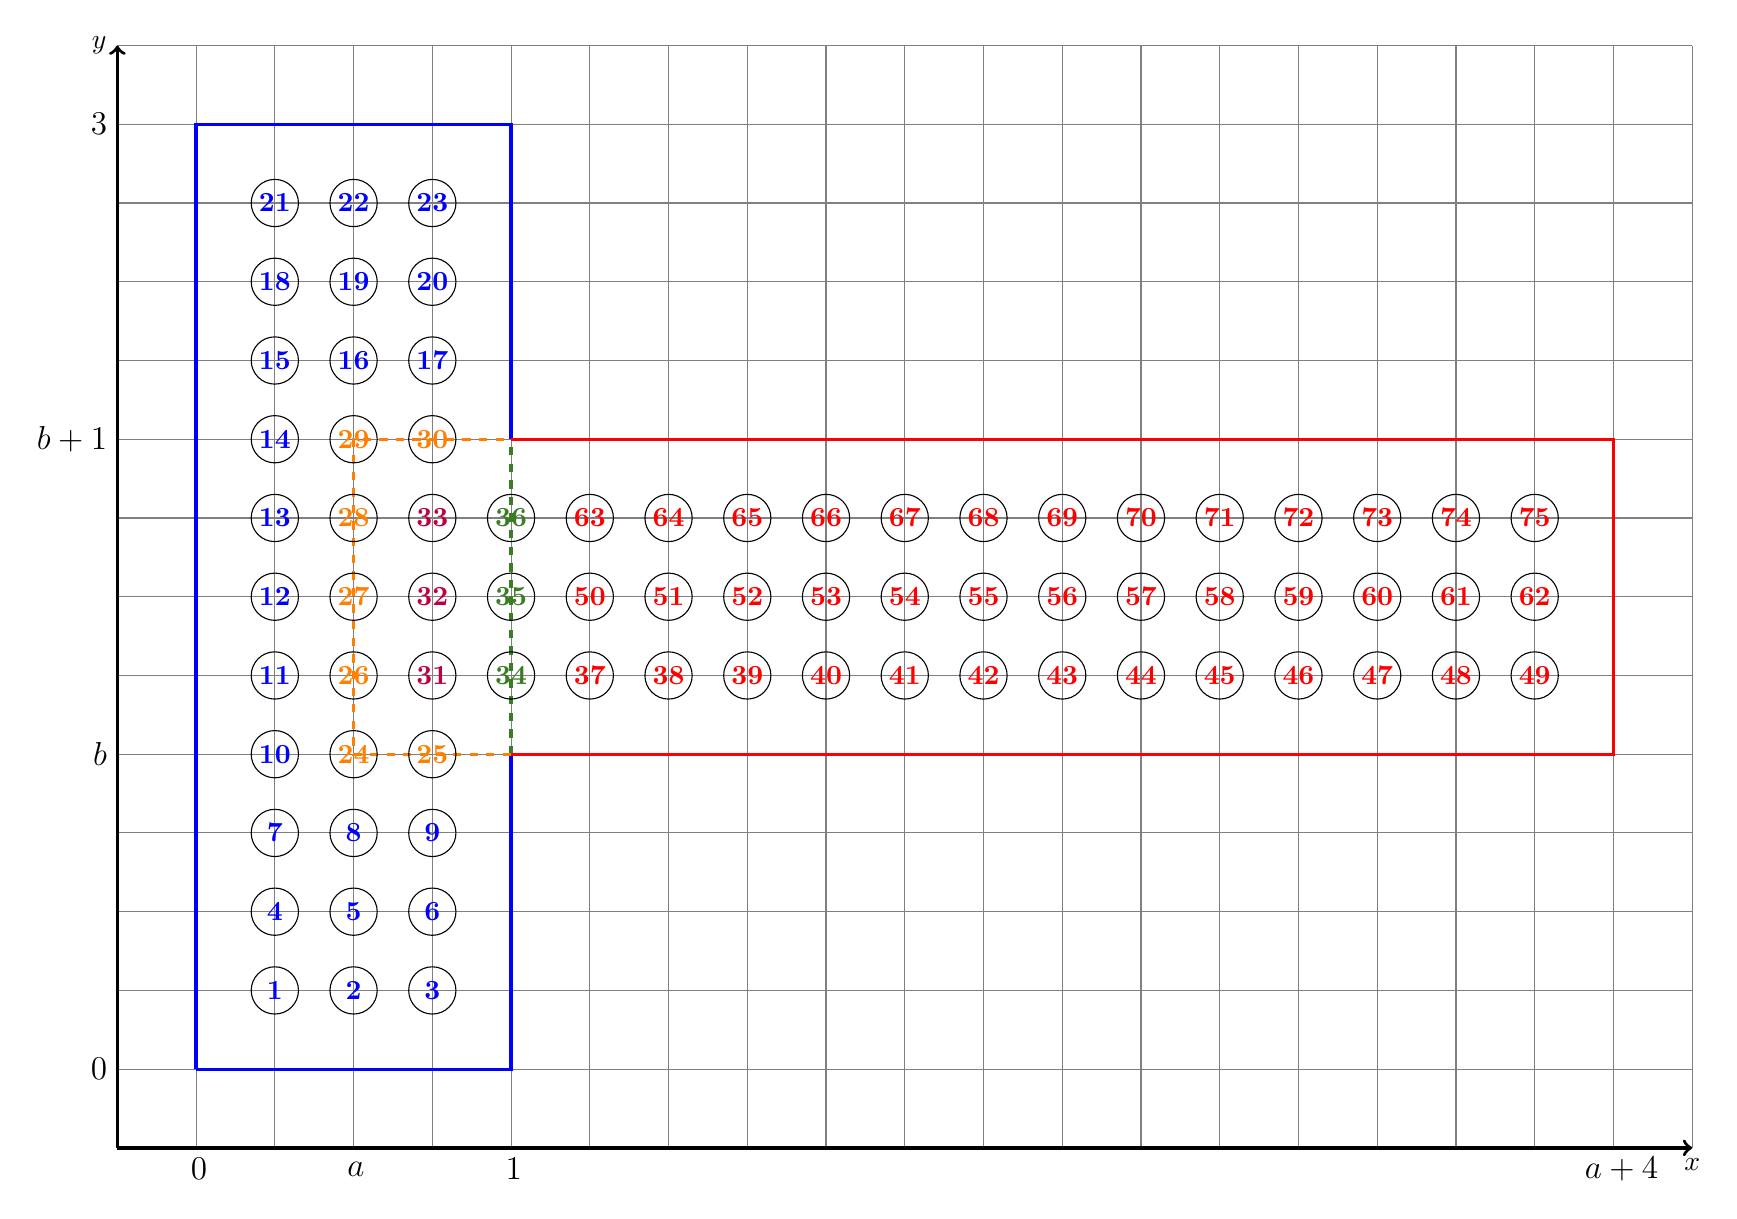
\begin{tikzpicture}
\draw[step=1cm,gray] (-1,-1) grid (19,13);
\draw[blue,very thick] (0,0) -- (4,0) -- (4,4);
\draw[OliveGreen,very thick,dashed] (4,4) -- (4,8);
\draw[blue,very thick] (4,8) -- (4,12) -- (0,12) -- (0,0);
\draw[red,very thick] (4,8) -- (18,8) -- (18,4) -- (4,4);
\draw[orange,very thick,dashed] (4,4) -- (2,4) -- (2,8) -- (4,8);
\draw[black,very thick,->] (-1,-1) -- (19,-1) node[anchor=north]{$x$};
\draw[black,very thick,->] (-1,-1) -- (-1,13)node[anchor=east] {$y$};

\filldraw(0.27,-1.27) node[circle, inner sep = 0pt, fill=white, minimum size = 0pt, label = left: {\large $\color{black} 0$}]{}; {};
\filldraw(2.27,-1.27) node[circle, inner sep = 0pt, fill=white, minimum size = 0pt, label = left: {\large $\color{black} a$}]{}; {};
\filldraw(4.27,-1.27) node[circle, inner sep = 0pt, fill=white, minimum size = 0pt, label = left: {\large $\color{black} 1$}]{}; {};
\filldraw(18.7,-1.27) node[circle, inner sep = 0pt, fill=white, minimum size = 0pt, label = left: {\large $\color{black} a+4$}]{}; {};


\filldraw(-1,0) node[circle, inner sep = 0pt, fill=white, minimum size = 0pt, label = left: {\large $\color{black} 0$}]{}; {};
\filldraw(-1,4) node[circle, inner sep = 0pt, fill=white, minimum size = 0pt, label = left: {\large $\color{black} b$}]{}; {};
\filldraw(-1,8) node[circle, inner sep = 0pt, fill=white, minimum size = 0pt, label = left: {\large $\color{black} b+1$}]{}; {};
\filldraw(-1,12) node[circle, inner sep = 0pt, fill=white, minimum size = 0pt, label = left: {\large $\color{black} 3$}]{}; {};

\foreach \x in {1,2,3}
    \foreach \y in {1,2,3,4,5,6,7,8,9,10,11}
    {
    \draw (\x,\y) circle (0.3cm);
    }
    \fill (1,1) node {\textbf{\color{blue} 1}};
    \fill (2,1) node {\textbf{\color{blue} 2}};
    \fill (3,1) node {\textbf{\color{blue} 3}};
    \fill (1,2) node {\textbf{\color{blue} 4}};
    \fill (2,2) node {\textbf{\color{blue} 5}};
    \fill (3,2) node {\textbf{\color{blue} 6}};
    \fill (1,3) node {\textbf{\color{blue} 7}};
    \fill (2,3) node {\textbf{\color{blue} 8}};
    \fill (3,3) node {\textbf{\color{blue} 9}};
    \fill (1,4) node {\textbf{\color{blue} 10}};
    \fill (1,5) node {\textbf{\color{blue} 11}};
    \fill (1,6) node {\textbf{\color{blue} 12}};
    \fill (1,7) node {\textbf{\color{blue} 13}};
    \fill (1,8) node {\textbf{\color{blue} 14}};
    \fill (1,9) node {\textbf{\color{blue} 15}};
    \fill (2,9) node {\textbf{\color{blue} 16}};
    \fill (3,9) node {\textbf{\color{blue} 17}};
    \fill (1,10) node {\textbf{\color{blue} 18}};
    \fill (2,10) node {\textbf{\color{blue} 19}};
    \fill (3,10) node {\textbf{\color{blue} 20}};
    \fill (1,11) node {\textbf{\color{blue} 21}};
    \fill (2,11) node {\textbf{\color{blue} 22}};
    \fill (3,11) node {\textbf{\color{blue} 23}};
    \fill (2,4) node {\textbf{\color{orange} 24}};
    \fill (3,4) node {\textbf{\color{orange} 25}};
    \fill (2,5) node {\textbf{\color{orange} 26}};
    \fill (2,6) node {\textbf{\color{orange} 27}};
    \fill (2,7) node {\textbf{\color{orange} 28}};
    \fill (2,8) node {\textbf{\color{orange} 29}};
    \fill (3,8) node {\textbf{\color{orange} 30}};
    \fill (3,5) node {\textbf{\color{purple} 31}};
    \fill (3,6) node {\textbf{\color{purple} 32}};
    \fill (3,7) node {\textbf{\color{purple} 33}};

\foreach \x in {4,5,6,7,8,9,10,11,12,13,14,15,16,17}
	\foreach \y in {5,6,7}
	{
	\draw (\x,\y) circle (0.3cm);
	}
	\fill (4,5) node {\textbf{\color{OliveGreen} 34}};
    \fill (4,6) node {\textbf{\color{OliveGreen} 35}};
    \fill (4,7) node {\textbf{\color{OliveGreen} 36}};
    	\fill (5,5) node {\textbf{\color{red} 37}};
    \fill (6,5) node {\textbf{\color{red} 38}};
    \fill (7,5) node {\textbf{\color{red} 39}};
    	\fill (8,5) node {\textbf{\color{red} 40}};
    \fill (9,5) node {\textbf{\color{red} 41}};
    \fill (10,5) node {\textbf{\color{red} 42}};
    \fill (11,5) node {\textbf{\color{red} 43}};
    \fill (12,5) node {\textbf{\color{red} 44}};
    \fill (13,5) node {\textbf{\color{red} 45}};
    	\fill (14,5) node {\textbf{\color{red} 46}};
    \fill (15,5) node {\textbf{\color{red} 47}};
    \fill (16,5) node {\textbf{\color{red} 48}};
    \fill (17,5) node {\textbf{\color{red} 49}};
    	\fill (5,6) node {\textbf{\color{red} 50}};
    \fill (6,6) node {\textbf{\color{red} 51}};
    \fill (7,6) node {\textbf{\color{red} 52}};
    	\fill (8,6) node {\textbf{\color{red} 53}};
    \fill (9,6) node {\textbf{\color{red} 54}};
    \fill (10,6) node {\textbf{\color{red} 55}};
    \fill (11,6) node {\textbf{\color{red} 56}};
    \fill (12,6) node {\textbf{\color{red} 57}};
    \fill (13,6) node {\textbf{\color{red} 58}};
    	\fill (14,6) node {\textbf{\color{red} 59}};
    \fill (15,6) node {\textbf{\color{red} 60}};
    \fill (16,6) node {\textbf{\color{red} 61}};
    \fill (17,6) node {\textbf{\color{red} 62}};
    	\fill (5,7) node {\textbf{\color{red} 63}};
    \fill (6,7) node {\textbf{\color{red} 64}};
    \fill (7,7) node {\textbf{\color{red} 65}};
    	\fill (8,7) node {\textbf{\color{red} 66}};
    \fill (9,7) node {\textbf{\color{red} 67}};
    \fill (10,7) node {\textbf{\color{red} 68}};
    \fill (11,7) node {\textbf{\color{red} 69}};
    \fill (12,7) node {\textbf{\color{red} 70}};
    \fill (13,7) node {\textbf{\color{red} 71}};
    	\fill (14,7) node {\textbf{\color{red} 72}};
    \fill (15,7) node {\textbf{\color{red} 73}};
    \fill (16,7) node {\textbf{\color{red} 74}};
    \fill (17,7) node {\textbf{\color{red} 75}};
\end{tikzpicture}
\caption{Part 3 Sample Grid Enumeration}
\end{figure}

\subsection{(a) Generate Data}\begin{mybox}{Cerulean}{}
Write Matlab programs that generate the "data" $A$ and $b$ of the discretized version,
$$Av = b,$$
of (1), as well as the submatrices $A_1$ and $A_2$ of $A$ corresponding to the subregions $R_1$ and $R_2$, respectively.  Design your program such that you can use any functions $f: R \to \R$ and $g: \partial R \to \R$.\\
\end{mybox}\text{ }\\

In order to create an enumeration matrix for $R_1$ and $R_2$ with matching grid points, I started by creating a matrix of dimension $length(h:h:a+4-h)\times length(h:h:3-h)$, corresponding to the region $R$, where $h = \frac{1}{2^m}$ denotes the grid size and $0 < a < 1$ is a parameter.  This matrix is used for the enumeration of our grid points, so I then went through and filled the matrix with the grid numbering shown below.  It is similar to how we numbered the grid points in $R_1$ and $R_2$ in class, except I chose to go by row, instead of by column.  Also note, that the enumeration matrix, $"Num\_Mat"$, is rotated 90 degrees to the right compared with the diagram below.  This decision was made to make indexing into the enumeration matrix more intuitive in future steps.  I then padded all four sizes of the matrix with zeros to signify the boundaries of $R_1$ and $R_2$.\\

\noindent
The diagram above is an illustration for $m = 2$, $a = \frac{1}{2}$, and $b = 1$.  The solid blue lines indicate {\color{blue}$\Sigma_1$}, the boundary of {\color{blue}$R_1$}; the dashed blue line indicates {\color{OliveGreen}$\Gamma_1$}, the artificial boundary of {\color{blue}$R_1$} within {\color{red}$R_2$}; the solid red lines indicate {\color{red}$\Sigma_2$}, the boundary of {\color{red}$R_2$}; and the dashed red lines indicate {\color{orange}$\Gamma_2$}, the artificial boundary of {\color{red}$R_2$} within {\color{blue}$R_1$}.  Furthermore, the blue dots corresponded to the interior points of {\color{blue}$R_1$} and the artificial boundary points of {\color{blue}$R_1$}, red dots correspond to the interior points of {\color{red}$R_2$} and the artificial boundary points of {\color{red}$R_2$}, and the purple pots correspond to points in the interior of {\color{purple}$R_1 \cap R_2$}.\\

\noindent
The reason for ordering the points in this way is so that we can ensure the vector $v$ will be in the order:
$$v = \begin{bmatrix}
{\color{blue}v_{R_1\backslash \overline{R}_2}} \\
{\color{orange}v_{\Gamma_2}} \\
{\color{purple}v_{R_1 \cap R_2}} \\
{\color{OliveGreen}v_{\Gamma_1}} \\
{\color{red}v_{R_2\backslash \overline{R}_1}} \\
\end{bmatrix}.$$

\noindent
After creating the enumeration matrix for each of the three cases ($b = 0$, $0 < b < 2$, and $b = 2$) I used this to construct $A$ by going point-by-point, and doing the 5-point stencil, i.e., for each point, I put a 4 in its corresponding location in $A$, and then found the numbers of the four closest points and put a -1 in their corresponding locations in $A$.  If ones of the four closest points was on the boundary of $R_1$ or $R_2$, then I added $g(x,y)$ at the index of the points location to $b$.  Where $b$ was initialized to equal $h^2f(x,y)$.  After generating $A$, it followed easily to extract $A_1$ and $A_2$ corresponding to $R_1$ and $R_2$ respectively.

\noindent
*\underline{Note:} For clarity, in my code I have change $a$ and $b$ to $c$ and $d$ respectively since we use "little b" in several other places.

\lstset{language=matlab,frame=single}
\begin{lstlisting}[caption=Enumeration for b equals 0]
function [Num_Mat,tot_R1_pts,tot_R2_pts,tot_pts,R1_xind,R1_yind,R2_xind,...
    R2_yind] = NumberedMatd0(m,c,d)

h = 1/(2^m);

x = h:h:c+4-h;
y = h:h:3-h;

nx = length(x);
ny = length(y);

Num_Mat = zeros(nx,ny);

% part of R1 to the left of R2
xLen_1 = (2^m)*c - 1;
yLen_1 = 2^m;

vec_1 = 1:xLen_1*yLen_1;
mat_1 = reshape(vec_1,[xLen_1,yLen_1]);
Num_Mat(1:xLen_1,1:yLen_1) = mat_1;

R1_pts = length(vec_1);

% part of R1 above R2
xLen_2 = 2^m - 1;
yLen_2 = 2*(2^m - 1) + 1;

vec_2 = vec_1(end) + 1: vec_1(end) + xLen_2*yLen_2;
mat_2 = reshape(vec_2,[xLen_2,yLen_2]);
Num_Mat(1:xLen_2,yLen_1 + 1:yLen_1 + yLen_2) = mat_2;

R1_pts = R1_pts + length(vec_2);

% long part of gamma2
xLen_gamma2_1 = 1;
yLen_gamma2_1 = 2^m;

vec_gamma2_1 = vec_2(end) + 1:vec_2(end) + xLen_gamma2_1*yLen_gamma2_1;
Num_Mat(xLen_1 + 1,1:2^m) = vec_gamma2_1;

gamma2_pts = length(vec_gamma2_1);

% short part of gamma2
xLen_gamma2_2 = (2^m)*(1 - c) - 1;
yLen_gamma2_2 = 1;

vec_gamma2_2 = vec_gamma2_1(end) + 1:vec_gamma2_1(end) + ...
    xLen_gamma2_2*yLen_gamma2_2;
Num_Mat((2^m)*c+1:2^m - 1,2^m) = vec_gamma2_2.';

gamma2_pts = gamma2_pts + length(vec_gamma2_2);

% part where R1 intersects R2
xLen_3 = (2^m)*(1 - c) - 1;
yLen_3 = 2^m - 1;

vec_3 = vec_gamma2_2(end) + 1:vec_gamma2_2(end) + xLen_3*yLen_3;
mat_3 = reshape(vec_3,[xLen_3,yLen_3]);
Num_Mat((2^m)*c+1:2^m - 1,1:2^m - 1) = mat_3;

R1R2_pts = length(vec_3);

% gamma1 part
xLen_gamma1 = 1;
yLen_gamma1 = 2^m - 1;

vec_gamma1 = vec_3(end) + 1:vec_3(end) + xLen_gamma1*yLen_gamma1;
Num_Mat(2^m,1:2^m - 1) = vec_gamma1;

gamma1_pts = length(vec_gamma1);

% part of R2 sticking out of R1
xLen_4 = (2^m)*(c + 3) - 1;
yLen_4 = 2^m - 1;

vec_4 = vec_gamma1(end) + 1:vec_gamma1(end) + xLen_4*yLen_4;
mat_4 = reshape(vec_4,[xLen_4,yLen_4]);
Num_Mat(2^m + 1:end,1:2^m - 1) = mat_4;

R2_pts = length(vec_4);

% put zeros on boundary of Num_Mat
Num_Mat = [zeros(size(Num_Mat,1),1), Num_Mat , zeros(size(Num_Mat,1),1)];
Num_Mat = [zeros(1,size(Num_Mat,2)); Num_Mat ; zeros(1,size(Num_Mat,2))];

% total number of points
tot_R1_pts = R1_pts + gamma2_pts + R1R2_pts;
tot_R2_pts = R1R2_pts + gamma1_pts + R2_pts;
tot_pts = tot_R1_pts + tot_R2_pts - R1R2_pts;

% make vectors of indices of R1 and R2 points
R1_xind = 1 + (1:2^m - 1);
R1_yind = 1 + (1:ny);
R2_xind = 1 + ((2^m)*c+1:nx);
R2_yind = 1 + ((2^m)*d+1:(2^m)*(d+1)-1);
end
\end{lstlisting}

\lstset{language=matlab,frame=single}
\begin{lstlisting}[caption=Enumeration for b between 0 and 2]
function [Num_Mat,tot_R1_pts,tot_R2_pts,tot_pts,R1_xind,R1_yind,R2_xind,...
    R2_yind] = NumberedMatd1(m,c,d)

h = 1/(2^m);

x = h:h:c+4-h;
y = h:h:3-h;

nx = length(x);
ny = length(y);

Num_Mat = zeros(nx,ny);

% part of R1 below R2
xLen_1 = 2^m - 1;
yLen_1 = (2^m)*d-1;

vec_1 = 1:xLen_1*yLen_1;
mat_1 = reshape(vec_1,[xLen_1, yLen_1]);
Num_Mat(1:xLen_1,1:yLen_1) = mat_1;

R1_pts = length(vec_1);

% part of R1 to the left of R2
xLen_2 = (2^m)*c - 1;
yLen_2 = 2^m + 1;

vec_2 = vec_1(end)+1:vec_1(end) + xLen_2*yLen_2;
mat_2 = reshape(vec_2,[xLen_2,yLen_2]);
Num_Mat(1:xLen_2,yLen_1 + 1:yLen_1 + yLen_2) = mat_2;

R1_pts = R1_pts + length(vec_2);

% part of R1 above R2
xLen_3 = 2^m - 1;
yLen_3 = (2^m)*(2-d) - 1;

vec_3 = vec_2(end) + 1:vec_2(end) + xLen_3*yLen_3;
mat_3 = reshape(vec_3,[yLen_3,xLen_3]);
Num_Mat(1:xLen_3,yLen_1+ yLen_2 + 1:yLen_1 + yLen_2 + yLen_3) = mat_3;

R1_pts = R1_pts + length(vec_3);

% first part of gamma2
xLen_gamma2_1 = (2^m - 1) - ((2^m)*c - 1);
yLen_gamma2_1 = 1;

vec_gamma2_1 = vec_3(end) + 1:vec_3(end) + xLen_gamma2_1*yLen_gamma2_1;
Num_Mat(xLen_2 + 1:xLen_1,2^m*d) = vec_gamma2_1';

gamma2_pts = length(vec_gamma2_1);

% second part of gamma2
xLen_gamma2_2 = 1;
yLen_gamma2_2 = 2^m - 1;

vec_gamma2_2 = vec_gamma2_1(end) + 1:vec_gamma2_1(end) + ...
    xLen_gamma2_2*yLen_gamma2_2;
Num_Mat(xLen_2+1,yLen_1 + 2:yLen_1 +1 + yLen_gamma2_2) = vec_gamma2_2;

gamma2_pts = gamma2_pts + length(vec_gamma2_2);

% third part of gamma2
xLen_gamma2_3 = (2^m - 1) - ((2^m)*c - 1);
yLen_gamma2_3 = 1;

vec_gamma2_3 = vec_gamma2_2(end) + 1:vec_gamma2_2(end) + ...
    xLen_gamma2_3*yLen_gamma2_3;
Num_Mat(xLen_2 + 1:xLen_1,(2^m)*(d+1)) = vec_gamma2_3';

gamma2_pts = gamma2_pts + length(vec_gamma2_3);

% intersecting part of R1 and R2
xLen_4 = (2^m)*(1-c) - 1;
yLen_4 = 2^m - 1;

vec_4 = vec_gamma2_3(end) + 1:vec_gamma2_3(end) +xLen_4*yLen_4;
mat_4 = reshape(vec_4,[xLen_4,yLen_4]);
Num_Mat((2^m)*c+1:2^m-1,(2^m*d + 1):(2^m)*(d+1) - 1) = mat_4;

R1R2_pts = length(vec_4);

% gamma1
xLen_gamma1 = 1;
yLen_gamma1 = 2^m - 1;

vec_gamma1 = vec_4(end) + 1:vec_4(end) + xLen_gamma1*yLen_gamma1;
Num_Mat(2^m,(2^m*d + 1):(2^m)*(d+1) - 1) = vec_gamma1;

gamma1_pts = length(vec_gamma1);

% part of R2 sticking out
xLen_5 = (2^m)*(c+3) - 1;
yLen_5 = 2^m - 1;

vec_5 = vec_gamma1(end) + 1:vec_gamma1(end) + xLen_5*yLen_5;
mat_5 = reshape(vec_5,[xLen_5,yLen_5]);
Num_Mat(2^m + 1:end,(2^m)*d + 1:(2^m)*(d+1)-1) = mat_5;

R2_pts = length(vec_5);

% put zeros on boundary of Num_Mat
Num_Mat = [zeros(size(Num_Mat,1),1), Num_Mat , zeros(size(Num_Mat,1),1)];
Num_Mat = [zeros(1,size(Num_Mat,2)); Num_Mat ; zeros(1,size(Num_Mat,2))];

% total number of points
tot_R1_pts = R1_pts + gamma2_pts + R1R2_pts;
tot_R2_pts = R1R2_pts + gamma1_pts + R2_pts;
tot_pts = tot_R1_pts + tot_R2_pts - R1R2_pts;

% make vectors of indices of R1 and R2 points
R1_xind = 1 + (1:2^m - 1);
R1_yind = 1 + (1:ny);
R2_xind = 1 + ((2^m)*c+1:nx);
R2_yind = 1 + ((2^m)*d+1:(2^m)*(d+1)-1);
end
\end{lstlisting}

\lstset{language=matlab,frame=single}
\begin{lstlisting}[caption=Enumeration for b equals 2]
function [Num_Mat,tot_R1_pts,tot_R2_pts,tot_pts,R1_xind,R1_yind,R2_xind,...
    R2_yind] = NumberedMatd2(m,c,d)

h = 1/(2^m);

x = h:h:c+4-h;
y = h:h:3-h;

nx = length(x);
ny = length(y);

Num_Mat = zeros(nx,ny);

% part of R1 below R2
xLen_1 = 2^m - 1; 
yLen_1 = 2*(2^m - 1) + 1; 

vec_1 = 1:xLen_1*yLen_1;
mat_1 = reshape(vec_1,[xLen_1,yLen_1]);
Num_Mat(1:xLen_1,1:yLen_1) = mat_1;

R1_pts = length(vec_1);

% part of R1 to the left of R2
xLen_2 = (2^m)*c - 1; 
yLen_2 = 2^m; 

vec_2 = vec_1(end) + 1:vec_1(end) + xLen_2*yLen_2;
mat_2 = reshape(vec_2,[xLen_2,yLen_2]);
Num_Mat(1:(2^m)*c - 1,yLen_1 + 1:yLen_1 + yLen_2) = mat_2;

R1_pts = R1_pts + length(vec_2);

% short part of gamma2
xLen_gamma2_1 = (2^m)*(1 - c);
yLen_gamma2_1 = 1;

vec_gamma2_1 = vec_2(end) + 1:vec_2(end) + xLen_gamma2_1*yLen_gamma2_1;
Num_Mat((2^m)*c:2^m - 1,yLen_1 + 1) = vec_gamma2_1.';

gamma2_pts = length(vec_gamma2_1);

% long part of gamma2
xLen_gamma2_2 = 1;
yLen_gamma2_2 = 2^m - 1;

vec_gamma2_2 = vec_gamma2_1(end) + 1:vec_gamma2_1(end) + ...
    xLen_gamma2_2*yLen_gamma2_2;
Num_Mat((2^m)*c,yLen_1 + 2:3*(2^m - 1) + 2) = vec_gamma2_2;

gamma2_pts = gamma2_pts + length(vec_gamma2_2);

% part where R1 and R2 intersect
xLen_3 = (2^m)*(1 - c) - 1;
yLen_3 = 2^m - 1;

vec_3 = vec_gamma2_2(end) + 1:vec_gamma2_2(end) + xLen_3*yLen_3;
mat_3 = reshape(vec_3,[xLen_3,yLen_3]);
Num_Mat((2^m)*c + 1:2^m - 1,yLen_1 + 2:3*(2^m - 1) + 2) = mat_3;

R1R2_pts = length(vec_3);

% gamma1
xLen_gamma1 = 1;
yLen_gamma1 = 2^m - 1;

vec_gamma1 = vec_3(end) + 1:vec_3(end) + xLen_gamma1*yLen_gamma1;
Num_Mat(2^m,yLen_1 + 2:3*(2^m - 1) + 2) = vec_gamma1;

gamma1_pts = length(vec_gamma1);

% part of R2 sticking out of R1
xLen_4 = (2^m)*(c + 3) - 1;
yLen_4 = 2^m - 1;

vec_4 = vec_gamma1(end) + 1:vec_gamma1(end) + xLen_4*yLen_4;
mat_4 = reshape(vec_4,[xLen_4,yLen_4]);
Num_Mat(2^m + 1:end,yLen_1 + 2:3*(2^m - 1) + 2) = mat_4;

R2_pts = length(vec_4);

% put zeros on boundary of Num_Mat
Num_Mat = [zeros(size(Num_Mat,1),1), Num_Mat , zeros(size(Num_Mat,1),1)];
Num_Mat = [zeros(1,size(Num_Mat,2)); Num_Mat ; zeros(1,size(Num_Mat,2))];

% total number of points
tot_R1_pts = R1_pts + gamma2_pts + R1R2_pts;
tot_R2_pts = R1R2_pts + gamma1_pts + R2_pts;
tot_pts = tot_R1_pts + tot_R2_pts - R1R2_pts;

% make vectors of indices of R1 and R2 points
R1_xind = 1 + (1:2^m - 1);
R1_yind = 1 + (1:ny);
R2_xind = 1 + ((2^m)*c+1:nx);
R2_yind = 1 + ((2^m)*d+1:(2^m)*(d+1)-1);
end
\end{lstlisting}

\lstset{language=matlab,frame=single}
\begin{lstlisting}[caption=Construct Matrix $A$ and Vector $b$]
function [A,b,A1,A2,I1,I2,Num_Mat,tot_R1_pts,tot_R2_pts,tot_pts,R1_xind,...
    R1_yind,R2_xind,R2_yind] = AbData(m,c,d,alpha,beta,gamma)

if (0 < d && d < 2)
    [Num_Mat,tot_R1_pts,tot_R2_pts,tot_pts,R1_xind,R1_yind,R2_xind,...
        R2_yind] = NumberedMatd1(m,c,d);
elseif (d == 0)
    [Num_Mat,tot_R1_pts,tot_R2_pts,tot_pts,R1_xind,R1_yind,R2_xind,...
        R2_yind] = NumberedMatd0(m,c,d);
elseif (d== 2)
    [Num_Mat,tot_R1_pts,tot_R2_pts,tot_pts,R1_xind,R1_yind,R2_xind,...
        R2_yind] = NumberedMatd2(m,c,d);
end

h = 1/(2^m);

[X,Y]=meshgrid(0:h:c+4,0:h:3);
X = X'; Y = Y';

f = @(x,y) (beta^2)*(pi^2).*(y.^alpha).*sin(beta*pi.*x).*cos(gamma*pi.*y)...
          + (pi^2)*(gamma^2).*(y.^alpha).*sin(beta*pi.*x).*cos(gamma*pi.*y)...
          + 2*pi*alpha*gamma.*(y.^(alpha-1)).*sin(gamma*pi.*y).*sin(beta*pi.*x)...
          - (alpha - 1)*alpha.*(x.^(alpha - 2)).*cos(gamma*pi.*y).*sin(beta*pi.*x);

g = @(x,y) y.^(alpha).*sin(beta*pi*x).*cos(gamma*pi*y); % on the boundaries

% construct A and b
n = tot_pts;

A = 4*speye(n,n);
b = zeros(n,1);

for i=1:n
    [data_x,data_y] = find(Num_Mat == i);
    b(i) = h^2.*f(X(data_x,data_y),Y(data_x,data_y));
    
    % find the 4 closest points
    stencil = zeros(4,2);
    stencil(1,:) = [data_x, data_y + 1];
    stencil(2,:) = [data_x, data_y - 1];
    stencil(3,:) = [data_x + 1, data_y];
    stencil(4,:) = [data_x - 1, data_y];
    
    for j = 1:size(stencil,1)
        colInd = Num_Mat(stencil(j,1),stencil(j,2));
        if (colInd ~= 0) % then it is not a boundary
            A(i,colInd) = -1;
        elseif (colInd == 0) % then it is a boundary
            b(i) = b(i) + g(X(stencil(j,1),stencil(j,2)),...
                Y(stencil(j,1),stencil(j,2))); 
        end
    end
end

% now we need to get A1 and A2 from A
A1 = A(1:tot_R1_pts,1:tot_R1_pts);
A2 = A(tot_pts - tot_R2_pts + 1:end,tot_pts - tot_R2_pts + 1:end);

% construct I1 and I2
I1 = [speye(tot_R1_pts,tot_R1_pts), zeros(tot_R1_pts,tot_pts - tot_R1_pts)];
I2 = [zeros(tot_R2_pts,tot_pts - tot_R2_pts), speye(tot_R2_pts,tot_R2_pts)];

end
\end{lstlisting}


\subsection{(b) Multiplicative Schwarz and PCG Methods}\begin{mybox}{Cerulean}{}
For each of the following two domain decomposition methods, write a Matlab program that solves the discretized problem $Av = b$:
\begin{itemize}
\item[(1)] Multiplicative Schwarz method;
\item[(2)] CG method with additive Schwarz preconditioning.
\end{itemize}
The program for each of these methods should allow as inputs an arbitrary initial guess $v^{(0)}$ for the solution of $Av = b$, a "small" convergence tolerance, tol, for the domain decomposition method, and a large integer $n_{max}$ to be used as a safeguard against an excessive number of iterations of the domain decomposition method.\\
For method (2), apply the preconditioner $M$ from the left, i.e., solve
$$M^{-1}Av = M^{-1}b,$$
and employ Matlab's "pcg" function.\\
\end{mybox}\text{ }\\

Now that we have generated $A$ and $b$ from our enumeration matrix we can perform Multiplicative Schwarz and CG with additive Schwarz preconditioning.\\
\begin{itemize}
\item[(1)]  For Multiplicative Schwarz, at each step we will need to compute
\begin{align*}
v^{(n+\frac{1}{2})} &= v^{(n)} + I_1^TA_1^{-1}I_1(b - Av^{(n)}) \\
&= v^{(n)} + \left(I_1^TA_1^{-1}I_1\right)\overline{v} \\
&= v^{(n)} + I_1^TA_1^{-1}\left(I_1\overline{v}\right) \\
&= v^{(n)} + I_1^TA_1^{-1}\overline{v}_1
\end{align*}
and
\begin{align*}
v^{(n+1)} &= v^{(n+\frac{1}{2})} + I_2^TA_2^{-1}I_2(b - Av^{(n+\frac{1}{2})}) \\
&= v^{(n+\frac{1}{2})} + \left(I_2^TA_2^{-1}I_2\right)\overline{v} \\
&= v^{(n+\frac{1}{2})} + I_2^TA_2^{-1}\left(I_2\overline{v}\right) \\
&= v^{(n+\frac{1}{2})} + I_2^TA_2^{-1}\overline{v}_2
\end{align*}
where we will use our FFT-based fast elliptic solver to quickly compute the solve with $A_1$, $A_1^{-1}\overline{v}_1$, and the solve with $A_2$, $A_2^{-1}\overline{v}_2$.  The catch is, that $\overline{v}_1$ and $\overline{v}_2$ are vectors.  So before we can input either into our fast elliptic solver, we need to reshape them into matrices.  However, we can't just use Matlab's "reshape" because we need to maintain the order that we prescribed in our enumeration matrix.  This is done in the first part of the code "RiSolve".  Then, we can input the corresponding matrix in the fast elliptic solver, and a matrix is returned.  So now, we need to reshape the output matrix back into a vector, again corresponding to the ordering prescribed by our enumeration matrix.  This is done in the second part of the code "RiSolve".  We can then complete the n-th step of Multiple Schwarz.\\

\lstset{language=matlab,frame=single}
\begin{lstlisting}[caption=Multiplicative Schwarz Function]
function [v_ms,V_ms,u,NumSolvesR1,NumSolvesR2] = MS(tol,nmax,m,c,d,...
    alpha,beta,gamma)

[A,b,A1,A2,I1,I2,Num_Mat,tot_R1_pts,tot_R2_pts,tot_pts,R1_xind,R1_yind,...
    R2_xind,R2_yind] = AbData(m,c,d,alpha,beta,gamma);

n = length(b);
h = 1/(2^m);

v0 = zeros(length(b),1);
v_whole = v0;
NumSolvesR1 = 0;
NumSolvesR2 = 0;

for nn = 1:nmax
    
    if ((norm(A\b - v_whole)/norm(A\b - v0)) < tol)
        nn
        break;
    end
    
    s = I1*(b - A*v_whole);
    kmin = 1;
    kmax = tot_R1_pts;
    
    w = RiSolve(R1_xind,R1_yind,kmin,kmax,s,0,1,0,3,Num_Mat,m);
    NumSolvesR1 = NumSolvesR1 + 1;
    
    v_half = v_whole + (I1.')*w;
    
    s = I2*(b - A*v_half);
    kmin = tot_pts - tot_R2_pts + 1;
    kmax = tot_pts;
    
    w = RiSolve(R2_xind,R2_yind,kmin,kmax,s,c,4,d,1,Num_Mat,m);
    NumSolvesR2 = NumSolvesR2 + 1;
    
    v_whole = v_half + (I2.')*w;
end

v_ms = v_whole; % this is a vector
n = length(b);
V_ms = zeros(size(Num_Mat,1),size(Num_Mat,2));

for i = 1:n
    [data_x,data_y] = find(Num_Mat == i);
    V_ms(data_x,data_y) = v_ms(i); 
end
    
x=0:h:c+4;
y=0:h:3;
[X,Y] = meshgrid(x,y);
X= X'; Y = Y';
u = zeros(size(Num_Mat));
for i=1:n
   [data_x,data_y] = find(Num_Mat == i);
   u(data_x,data_y) = Y(data_x,data_y).^(alpha).*...
       sin(beta*pi*X(data_x,data_y)).*cos(gamma*pi*Y(data_x,data_y));
end
end
\end{lstlisting}

\lstset{language=matlab,frame=single}
\begin{lstlisting}[caption=Fast Elliptic Solver on $R_i$]
function w = RiSolve(Ri_xind,Ri_yind,kmin,kmax,s,c,ic,d,id,Num_Mat,m)

W = zeros(size(Num_Mat));
% reshape to a matrix
for k = 1:(kmax - kmin + 1)
    [data_x,data_y] = find(Num_Mat == (kmin + k - 1));
    W(data_x,data_y) = s(k);
end

% put into fft solver
W(Ri_xind,Ri_yind) = fft2DPoisson(m,W(Ri_xind,Ri_yind),c,ic,d,id);

w = zeros(length(s),1);
% reshape into vector
for k = 1:(kmax - kmin + 1)
    [data_x,data_y] = find(Num_Mat == (kmin + k - 1));
    w(k) = W(data_x,data_y);
end
end
\end{lstlisting} \text{ }\\


\item[(2)] For CG with additive Schwarz preconditioning, we use $M:=(B_1 + B_2)^{-1}$ as a preconditioner, where $B_i = I_i^TA_i^{-1}I_i$.  To do this, it is more efficient for us to write a solver to compute $q = A'v$, where $A' = M^{-1}A$, and use the function handle as an input for Matlab's "pcg", than it is to just input $A$ and $M$ into "pcg".  This is because we can, again, employ our fast elliptic solver from Part 1.  We do this as follows:
\begin{align*}
A'v &= M^{-1}Av \\
&= (B_1 + B_2)Av \\
& = (B_1 + B_2)\overline{v} \\
&= B_1\overline{v} + B_2\overline{v} \\
&= \left(I_1^TA_1^{-1}I_1\right)\overline{v} + \left(I_2^TA_2^{-1}I_2\right)\overline{v} \\
&= \left(I_1^TA_1^{-1}\right)\left(I_1\overline{v}\right) + \left(I_2^TA_2^{-1}\right)\left(I_2\overline{v}\right) \\
&= I_1^T\underbrace{\left(A_1^{-1}s_1\right)}_{(*1)} + I_2^T\underbrace{\left(A_2^{-1}s_2\right)}_{(*2)} 
\end{align*}
where (*1) and (*2) can be solved using our fast elliptic solver, with the same procedure outlined for Multiplicative Schwarz, using the code "RiSolve" to reshape the vector into a matrix, plug into the fast elliptic solver, and then reshape back into a vector.  Similarly, for $b'$, we have:
\begin{align*}
b' &= M^{-1}b \\
&= (B_1 + B_2)b \\
&= B_1b + B_1b \\
&= \left(I_1^TA_1^{-1}I_1\right)b + \left(I_2^TA_2^{-1}I_2\right)b \\
&= \left(I_1^TA_1^{-1}\right)\left(I_1b\right) + \left(I_2^TA_2^{-1}\right)\left(I_2b\right) \\
&= I_1^T\underbrace{\left(A_1^{-1}w_1\right)}_{(*3)} + I_2^T\underbrace{\left(A_2^{-1}w_2\right)}_{(*4)}
\end{align*} 
where (*3) and (*4) can be solved using our fast elliptic solver.

\lstset{language=matlab,frame=single}
\begin{lstlisting}[caption=CG Method with Additive Schwarz Preconditioner]
function [v_pcgs,V_pcgs,u,NumSolvesR1,NumSolvesR2] = PCGSchwarz(tol,nmax,...
    m,c,d,alpha,beta,gamma)

[A,b,A1,A2,I1,I2,Num_Mat,tot_R1_pts,tot_R2_pts,tot_pts,R1_xind,R1_yind,...
    R2_xind,R2_yind] = AbData(m,c,d,alpha,beta,gamma);

v0 = zeros(length(b),1);

h = 1/(2^m);
n = length(b);

v0p = v0;
% compute b'=M^-1*b
s1 = I1*b;
s2 = I2*b;
kmin1 = 1;
kmax1 = tot_R1_pts;
w1 = RiSolve(R1_xind,R1_yind,kmin1,kmax1,s1,0,1,0,3,Num_Mat,m);
NumSolvesR1 = 1;
kmin2 = tot_pts - tot_R2_pts + 1;
kmax2 = tot_pts;
w2 = RiSolve(R2_xind,R2_yind,kmin2,kmax2,s2,0,4,0,1,Num_Mat,m);
NumSolvesR2 = 1;
bp = (I1.')*w1 + (I2.')*w2;


v_pcgs = pcg(@(v) ApMult(A,v),bp,tol,nmax,[],[],v0p);

V_pcgs = zeros(size(Num_Mat,1),size(Num_Mat,2));

for i = 1:n
    [data_x,data_y] = find(Num_Mat == i);
    V_pcgs(data_x,data_y) = v_pcgs(i); 
end

x=0:h:c+4;
y=0:h:3;
[X,Y] = meshgrid(x,y);
X= X'; Y = Y';
u = zeros(size(Num_Mat));
for i=1:n
   [data_x,data_y] = find(Num_Mat == i);
   u(data_x,data_y) = Y(data_x,data_y).^(alpha).*...
       sin(beta*pi*X(data_x,data_y)).*cos(gamma*pi*Y(data_x,data_y));
end

% function to compute q = A'p
    function q = ApMult(A,v)
        v_bar = A*v;
        s1 = I1*v_bar;
        s2 = I2*v_bar;
        kmin1 = 1;
        kmax1 = tot_R1_pts;
        w1 = RiSolve(R1_xind,R1_yind,kmin1,kmax1,s1,0,1,0,3,Num_Mat,m);
        kmin2 = tot_pts - tot_R2_pts + 1;
        kmax2 = tot_pts;
        w2 = RiSolve(R2_xind,R2_yind,kmin2,kmax2,s2,0,4,0,1,Num_Mat,m);
        q = (I1.')*w1 + (I2.')*w2;
        NumSolvesR1 = NumSolvesR1 + 1;
        NumSolvesR2 = NumSolvesR2 + 1;
    end
end
\end{lstlisting}

\end{itemize}


\newpage
\subsection{(c) Test Program}\begin{mybox}{Cerulean}{}
To test each of your programs, choose the functions $f$ and$g$ such that
\begin{align*}
u(x,y) = y^\alpha\sin(\beta\pi x)\cos(\gamma\pi y), \tag{4}
\end{align*}
where $\alpha \geq 0$ and $\beta, \gamma > 0$ are parameters, is the exact solution of problem (1).  Note that this family of functions was also used in Problem 1 of Homework 3.\\
Run the following 6 cases:
\begin{itemize}
\item[(i)] $a = \frac{1}{2}$, $b = 0$, $\alpha = 0$, $\beta = 1$, $\gamma = \frac{1}{2}$;
\item[(ii)] $a = \frac{1}{2}$, $b = 0$, $\alpha = 2$, $\beta = \frac{7}{2}$, $\gamma = 2$;
\item[(iii)] $a = \frac{1}{4}$, $b = 1$, $\alpha = 0$, $\beta = 1$, $\gamma = \frac{1}{2}$;
\item[(iv)] $a = \frac{1}{4}$, $b = 1$, $\alpha = 2$, $\beta = \frac{7}{2}$, $\gamma = 2$;
\item[(v)] $a = \frac{1}{2}$, $b = 2$, $\alpha = 0$, $\beta = 1$, $\gamma = \frac{1}{2}$;
\item[(vi)] $a = \frac{1}{2}$, $b = 2$, $\alpha = 2$, $\beta = \frac{7}{2}$, $\gamma = 2$;
\end{itemize}
Here, $a$, $b$ and $\alpha$, $\beta$, $\gamma$ are the parameters in (2) and (4), respectively.\\
For each of these 6 cases, run both methods (1) and (2).  Thus there is a total of 12 runs.\\
For each of your runs, determine the relative maximum error of your computed approximate solution at the grid points:
\begin{align*}
\frac{\max_{j,k}|v_{jk} - u(x_j,y_k)|}{\max_{j,k}|u(x_j,y_k)|} \tag{5}
\end{align*}
Here, $v_{jk}$ denotes the computed approximate solution at the grid point $(x_j,y_k)$, and the maximum is taken over all grid points.  For each run, choose $m$ in the grid spacing (3) large enough and the convergence tolerance, tol, small enough so that the relative maximal error (5) is below $5\times 10^{-4}$.  For each run, print out the $m$ you have used, the corresponding values of (5), and the total numbers of solves on $R_1$ and solves on $R_2$ used in the domain decomposition method.  For each run, submit a three-dimensional plot of the computed solution $v_{jk}$.\\
Comment on your results and the efficiency of methods (1) and (2).
\end{mybox}\text{ }\\

\newpage
\lstset{language=matlab,frame=single}
\begin{lstlisting}[caption=Part 3 Example Run]
% case(i): c=1/2, d=0, alpha=0, beta=1, gamma=1/2
m = 6; c = 1/2; d = 0; alpha = 0; beta = 1; gamma = 1/2; %m=6
h = 1/(2^m);
tol = 1e-6;
nmax = 100;
[v_ms,V_ms,u,NumSolvesR1,NumSolvesR2] = MS(tol,nmax,m,c,d,alpha,beta,gamma);
NumSolvesR1
NumSolvesR2

% plot ms
x=0:h:c+4;
y=0:h:3; 
[X,Y] = meshgrid(x,y);
X= X'; Y = Y';

errorims = max(max(abs(V_ms - u)))/max(max(abs(u)))

subplot(3,4,1) 
surf(X,Y,V_ms,'Edgecolor','none')
colorbar
title('Case (i): Multiplicative Schwarz')

[v_pcgs,V_pcgs,u,NumSolvesR1,NumSolvesR2] = PCGSchwarz(tol,nmax,m,c,d,...
    alpha,beta,gamma);
NumSolvesR1
NumSolvesR2
erroripcgs = max(max(abs(V_pcgs - u)))/max(max(abs(u)))

%plot pcgs
subplot(3,4,2)
surf(X,Y,V_ms,'Edgecolor','none')
colorbar
title('Case (i): PCG Schwarz')
\end{lstlisting}

\begin{figure}[H]
\hspace{-1in}
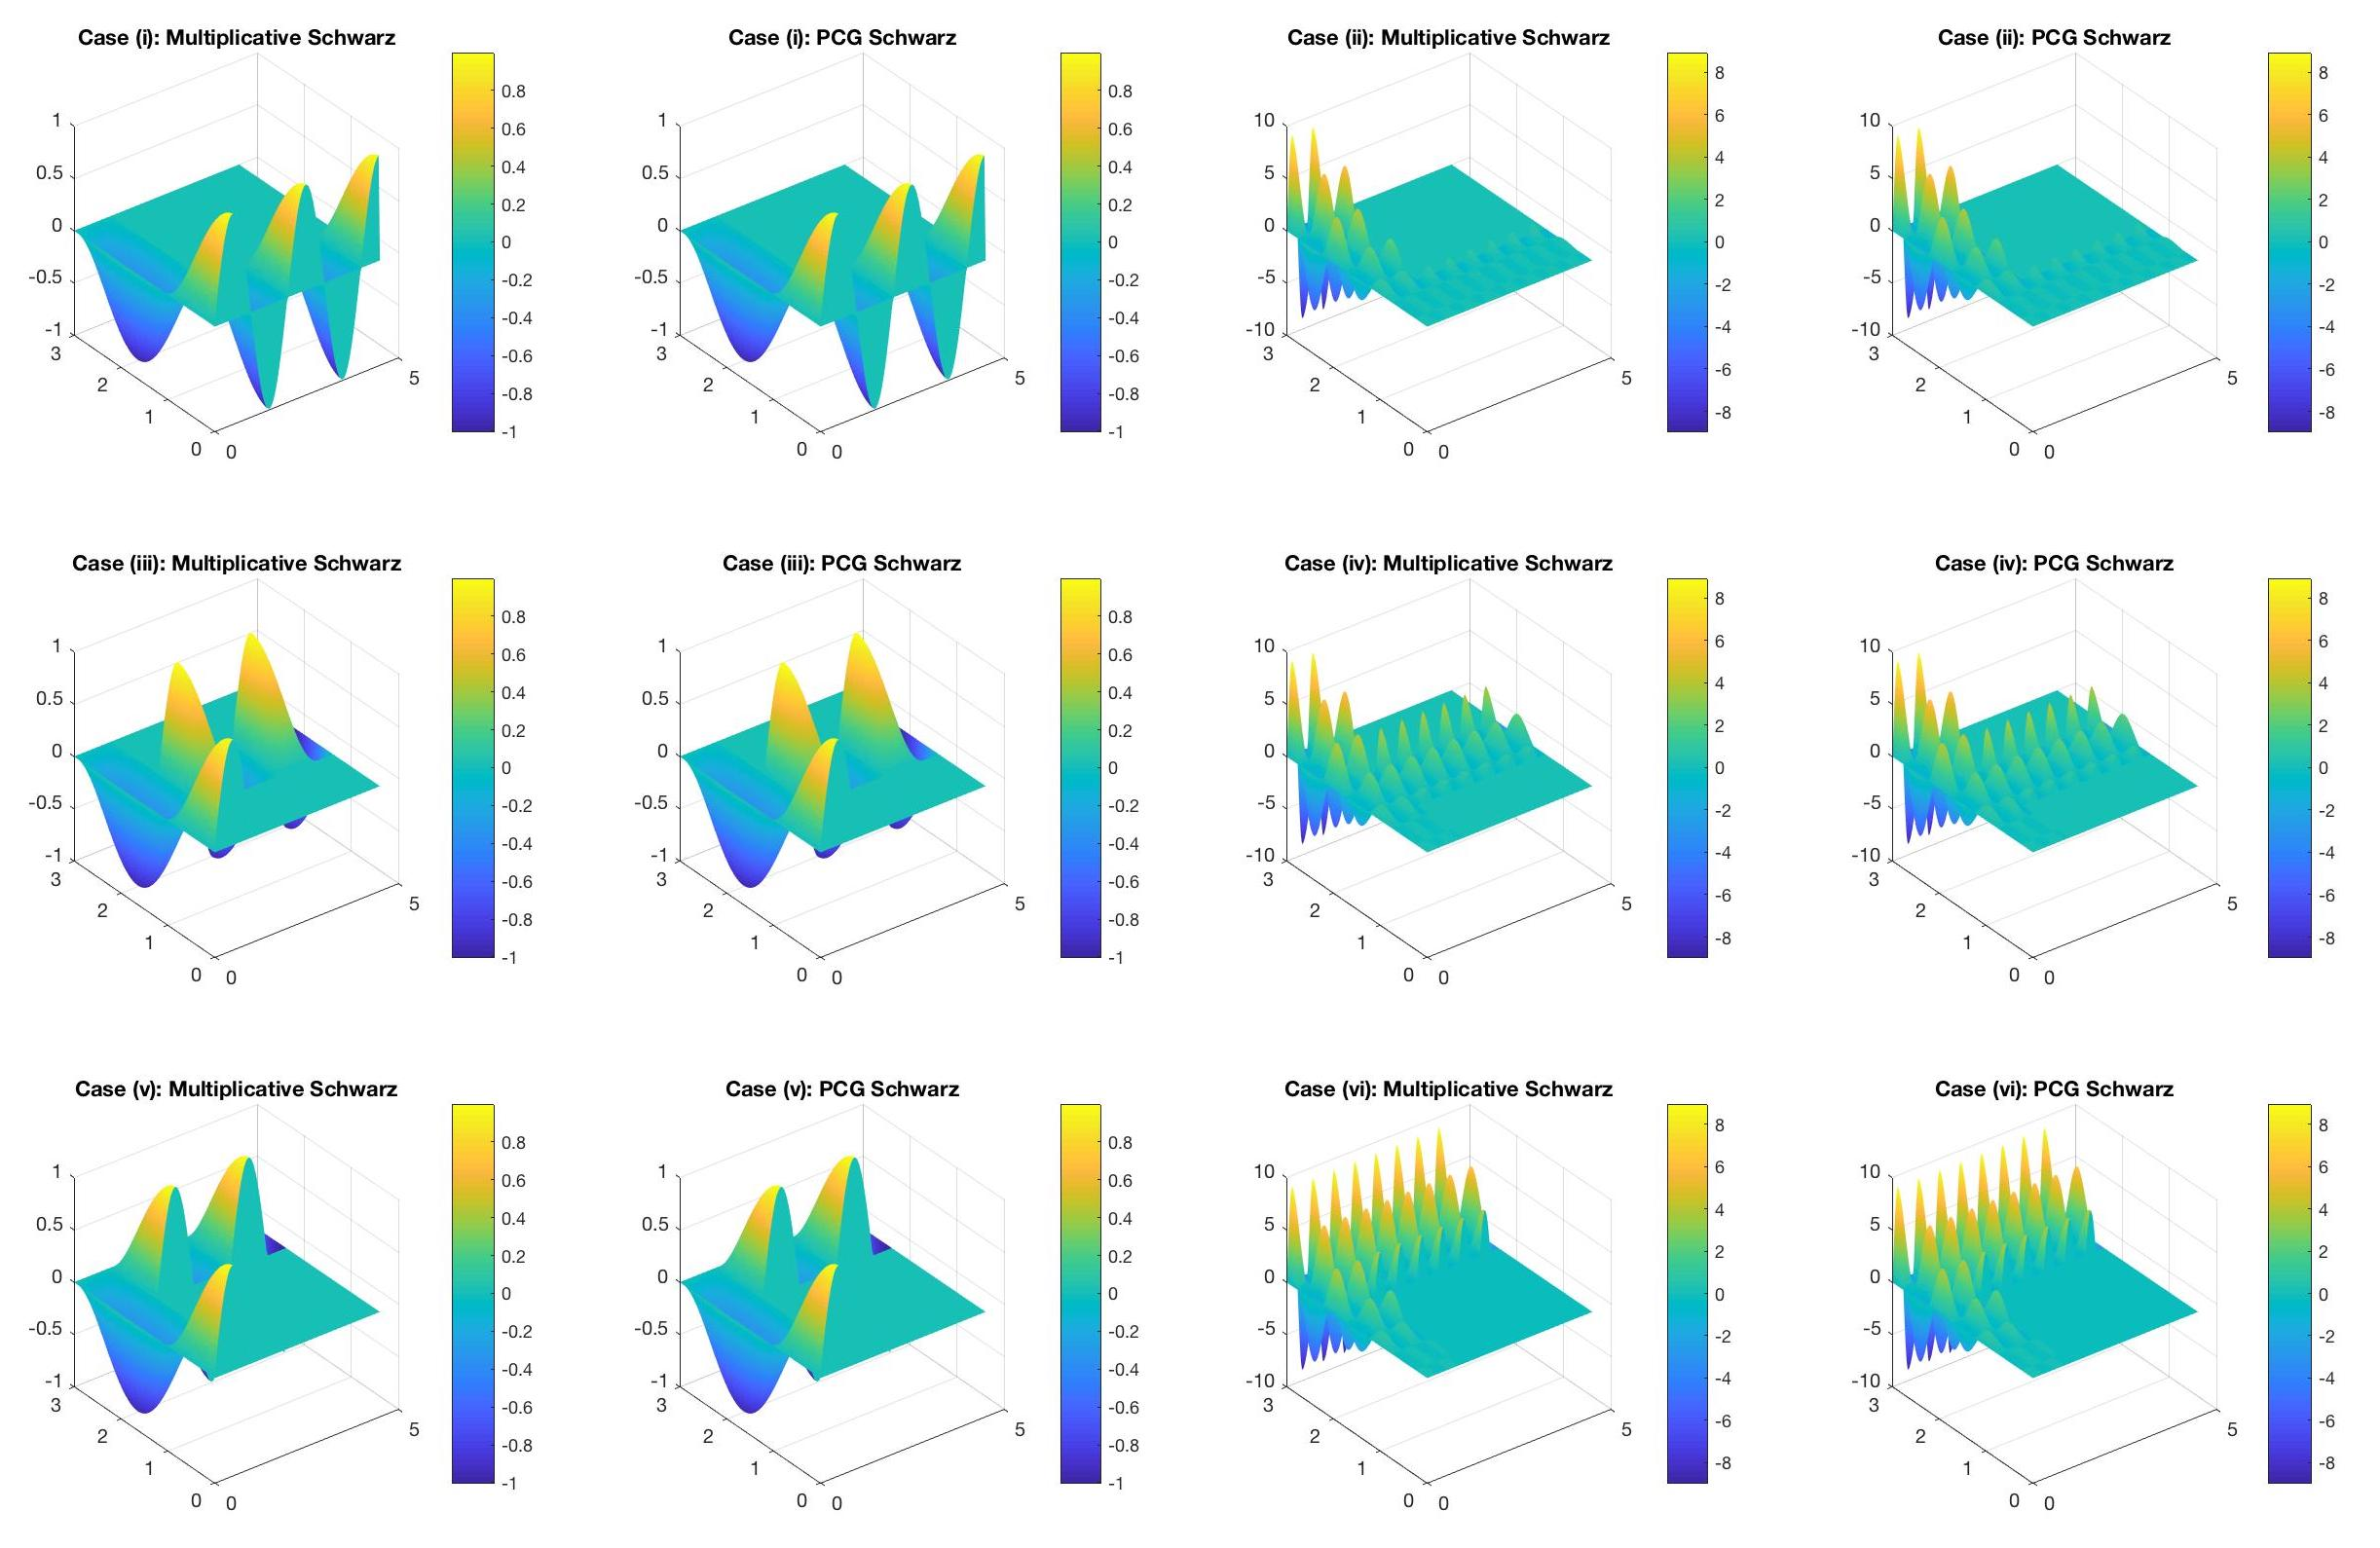
\includegraphics[scale=.25]{Part3_graphs.jpg}
\caption{Part 3 Surface Plots}
\end{figure}
*Note: The above is a portion of the my script to run and plot both my Multiplicative Schwarz and PCG with Additive Schwarz Preconditioner functions.  I only included Case (i) above as an example, because I did all 6 cases in an identical fashion, so it is unnecessary to include them all.


\begin{table}[H]
\centering
\renewcommand{\arraystretch}{1.3}
\begin{small}
\begin{tabular}{| c || c | c | c | c | c | c | c |}
\hline
\textbf{Case} & \textbf{Method} & \textbf{m} & \textbf{tol} & \textbf{nmax} &  \textbf{Error} & \textbf{$R_1$ Solves} & \textbf{$R_2$ Solves}\\
\hline 
\hline
(i)  & MS  & 6  & $10^{-6}$  & 100  & 1.710125682052865e-04  &  1 &  1 \\
  & PCGS  & 6  &  $10^{-6}$ & 100  & 1.705582642324011e-04  &  15 &  15 \\
\hline
(ii)  & MS  &  7 & $10^{-6}$  & 100  & 4.444357791847706e-04  & 7  &  7 \\
  & PCGS$^*$  & 6  &  $10^{-6}$ & 100  & 1.796278167890813e-03  & 11  & 11  \\
\hline
(iii)  & MS  & 6  & $10^{-6}$  & 100  & 1.766327631437248e-04  & 2  &  2 \\
  & PCGS  & 6  & $10^{-6}$  & 100  & 1.773632771441269e-04  & 24  & 24  \\
\hline
(iv)  &  MS & 7  & $10^{-6}$  & 100  & 4.440502127163036e-04  & 8  &  8 \\
  & PCGS$^*$  &  5 &  $10^{-6}$ & 100  & 7.359404861291871e-03  & 70  & 70  \\
\hline
(v)  & MS  & 6 & $10^{-6}$  & 100  & 1.762813820923581e-04  & 2  & 2  \\
  &  PCGS & 6  & $10^{-6}$  & 100  & 1.826466035048657e-04  & 21  & 21  \\
\hline
(vi)  & MS  &  7 &  $10^{-6}$ & 100  & 4.112264171431987e-04  & 7  & 7  \\
(vi)  & PCGS$^*$  &  6 & $10^{-6}$  & 100  &  1.669063601155044e-03 &  20 &  20 \\

\hline
\end{tabular}
\end{small}
\caption{Part 3 Results}
\end{table} 

* Relative maximal error was not below $5\times 10^{-4}$ regardless of tolerance or grid spacing, so the the results producing the smallest relative maximal error are listed.\\

As can be seen in the table above, for cases (i), (iii), and (v), Multiplicative Schwarz and CG with Additive Schwarz Preconditioner produces very similar results in terms of relative maximal error, however, MS requires significantly less solves on $R_1$ and $R_2$, making it faster and more efficient.  FOr cases (ii), (iv), and (vi), PCGS produces a higher relative maximal error regardless of $m$ value ( tried up to $m=7$, and the error got worse.  $m=8$ crashed Matlab).\\

\noindent
\underline{Note:} In my code you will notice that I wrote in my own counter for the number of solves on $R_1$ and the number of solves on $R_2$ in my PCGS function.  When I compared my number of iterations to the number of solves on $R_1$ and $R_2$, I expected them to be the same.  However, my counter always return something a little higher than the number of iterations.  This is because Matlab's "pcg" function includes some extra checks that requires solves on $R_1$ and $R_2$, that are not actually part of each iteration.  I assumed that it was not intended for those extra solves to be included in the recorded number of solves on $R_1$ and $R_2$, so the numbers in the above table are equivalent to the total number of iterations that "pcg" ran.

\newpage
\section{Part 4: Non-Matching Grids} \begin{mybox}{Cerulean}{}
In this part, we assume that neither $a$ nor $b$ in (2) are multiples of the spacing $h$, so that we do not have matching grids on $R_1$ and $R_2$.\\
\end{mybox}\text{ }\\

\begin{figure}[H]
\hspace{-1.1in}
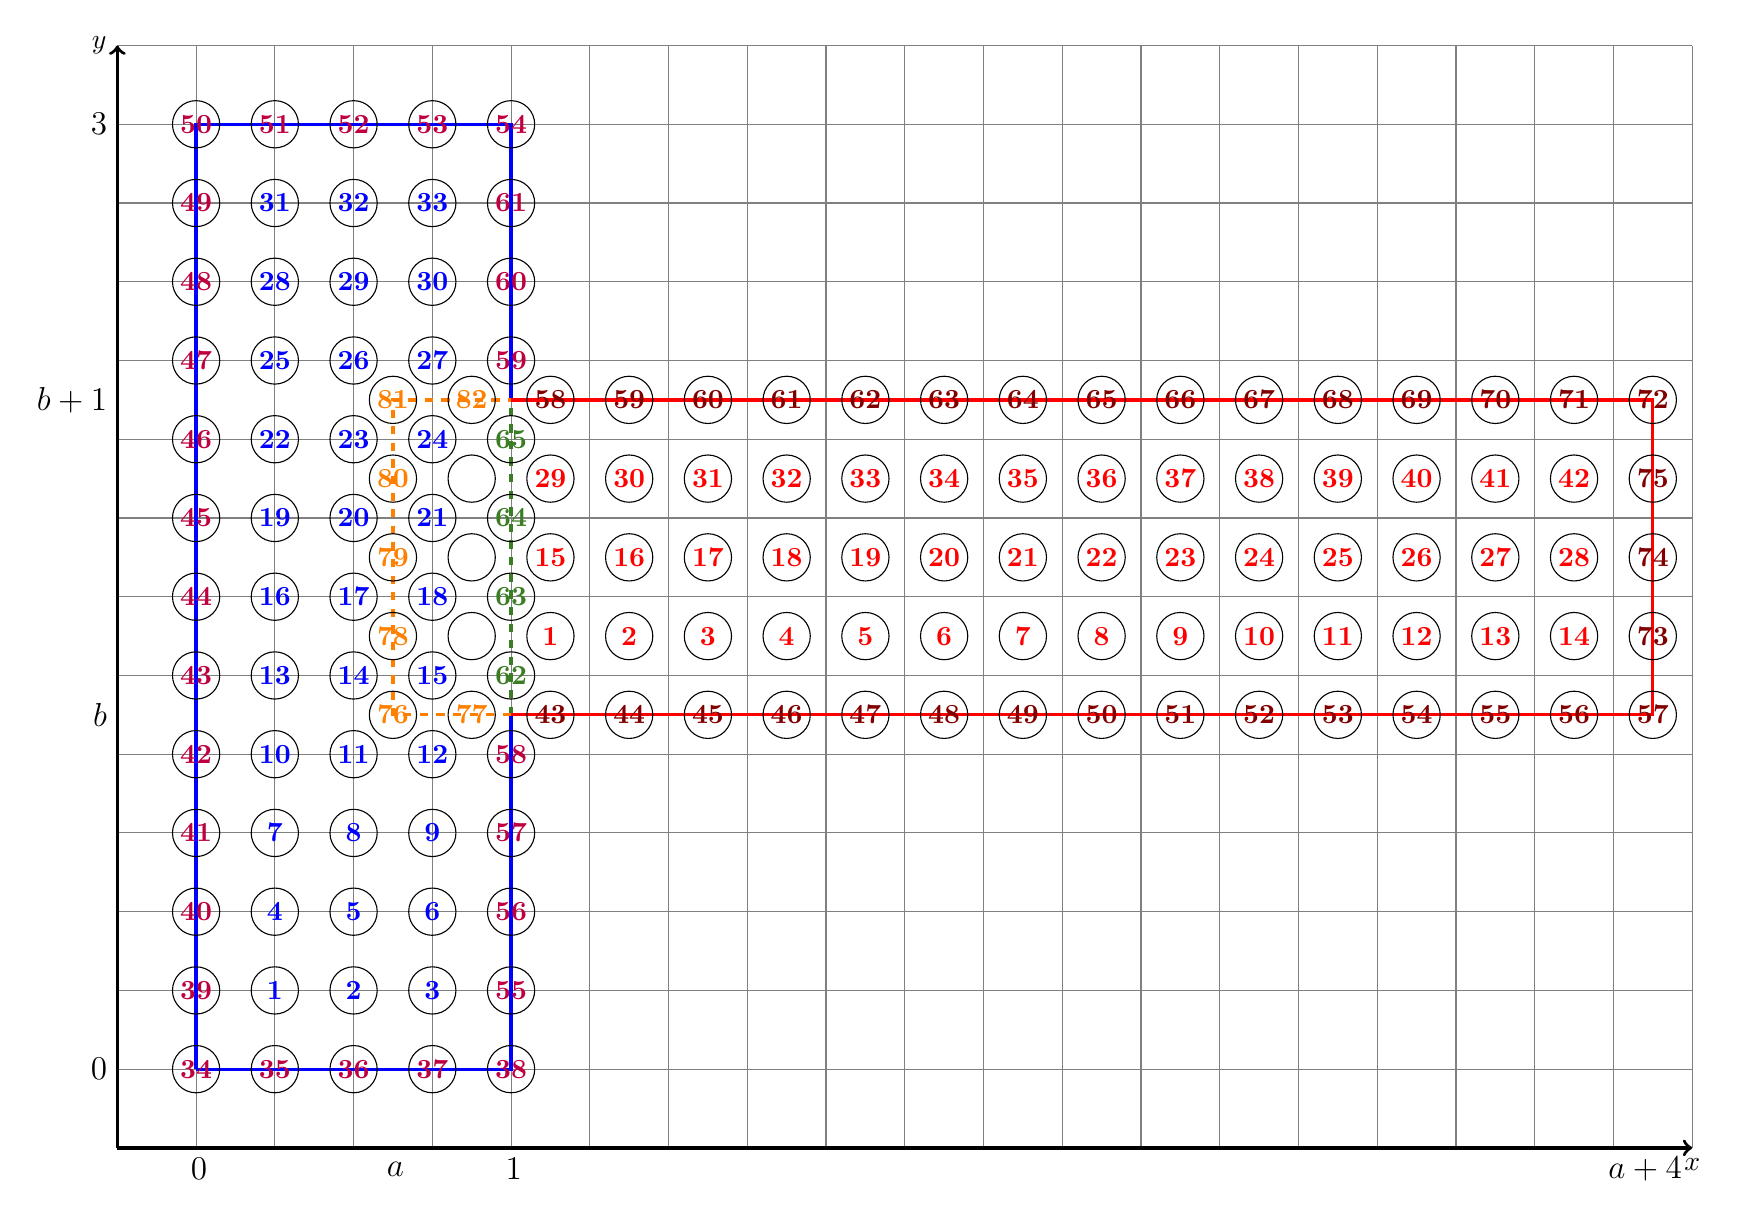
\begin{tikzpicture}
\draw[step=1cm,gray] (-1,-1) grid (19,13);
\draw[blue,very thick] (0,0) -- (4,0) -- (4,4.5);
\draw[OliveGreen,very thick,dashed] (4,4.5) -- (4,8.5);
\draw[blue,very thick] (4,8.5) -- (4,12) -- (0,12) -- (0,0);

\draw[red,very thick] (4,8.5) -- (18.5,8.5) -- (18.5,4.5) -- (4,4.5);
\draw[orange,very thick,dashed] (4,4.5) -- (2.5,4.5) -- (2.5,8.5) -- (4,8.5);

\draw[black,very thick,->] (-1,-1) -- (19,-1) node[anchor=north]{$x$};
\draw[black,very thick,->] (-1,-1) -- (-1,13)node[anchor=east] {$y$};

\filldraw(0.27,-1.27) node[circle, inner sep = 0pt, fill=white, minimum size = 0pt, label = left: {\large $\color{black} 0$}]{}; {};
\filldraw(2.77,-1.27) node[circle, inner sep = 0pt, fill=white, minimum size = 0pt, label = left: {\large $\color{black} a$}]{}; {};
\filldraw(4.27,-1.27) node[circle, inner sep = 0pt, fill=white, minimum size = 0pt, label = left: {\large $\color{black} 1$}]{}; {};
\filldraw(19,-1.27) node[circle, inner sep = 0pt, fill=white, minimum size = 0pt, label = left: {\large $\color{black} a+4$}]{}; {};


\filldraw(-1,0) node[circle, inner sep = 0pt, fill=white, minimum size = 0pt, label = left: {\large $\color{black} 0$}]{}; {};
\filldraw(-1,4.5) node[circle, inner sep = 0pt, fill=white, minimum size = 0pt, label = left: {\large $\color{black} b$}]{}; {};
\filldraw(-1,8.5) node[circle, inner sep = 0pt, fill=white, minimum size = 0pt, label = left: {\large $\color{black} b+1$}]{}; {};
\filldraw(-1,12) node[circle, inner sep = 0pt, fill=white, minimum size = 0pt, label = left: {\large $\color{black} 3$}]{}; {};

\foreach \x in {0,1,2,3,4}
    \foreach \y in {0,1,2,3,4,5,6,7,8,9,10,11,12}
    {
    \draw (\x,\y) circle (0.3cm);
    }
    \fill (1,1) node {\textbf{\color{blue} 1}};
    \fill (2,1) node {\textbf{\color{blue} 2}};
    \fill (3,1) node {\textbf{\color{blue} 3}};
    \fill (1,2) node {\textbf{\color{blue} 4}};
    \fill (2,2) node {\textbf{\color{blue} 5}};
    \fill (3,2) node {\textbf{\color{blue} 6}};
    \fill (1,3) node {\textbf{\color{blue} 7}};
    \fill (2,3) node {\textbf{\color{blue} 8}};
    \fill (3,3) node {\textbf{\color{blue} 9}};
    \fill (1,4) node {\textbf{\color{blue} 10}};
    \fill (2,4) node {\textbf{\color{blue} 11}};
    \fill (3,4) node {\textbf{\color{blue} 12}};
    \fill (1,5) node {\textbf{\color{blue} 13}};
    \fill (2,5) node {\textbf{\color{blue} 14}};
    \fill (3,5) node {\textbf{\color{blue} 15}};
    \fill (1,6) node {\textbf{\color{blue} 16}};
    \fill (2,6) node {\textbf{\color{blue} 17}};
    \fill (3,6) node {\textbf{\color{blue} 18}};
    \fill (1,7) node {\textbf{\color{blue} 19}};
    \fill (2,7) node {\textbf{\color{blue} 20}};
    \fill (3,7) node {\textbf{\color{blue} 21}};
    \fill (1,8) node {\textbf{\color{blue} 22}};
    \fill (2,8) node {\textbf{\color{blue} 23}};
    \fill (3,8) node {\textbf{\color{blue} 24}};
    \fill (1,9) node {\textbf{\color{blue} 25}};
    \fill (2,9) node {\textbf{\color{blue} 26}};
    \fill (3,9) node {\textbf{\color{blue} 27}};
    \fill (1,10) node {\textbf{\color{blue} 28}};
    \fill (2,10) node {\textbf{\color{blue} 29}};
    \fill (3,10) node {\textbf{\color{blue} 30}};
    \fill (1,11) node {\textbf{\color{blue} 31}};
    \fill (2,11) node {\textbf{\color{blue} 32}};
    \fill (3,11) node {\textbf{\color{blue} 33}};
    \fill (0,0) node {\textbf{\color{purple} 34}};
    \fill (1,0) node {\textbf{\color{purple} 35}};
    \fill (2,0) node {\textbf{\color{purple} 36}};
    \fill (3,0) node {\textbf{\color{purple} 37}};
    \fill (4,0) node {\textbf{\color{purple} 38}};
    \fill (0,1) node {\textbf{\color{purple} 39}};
    \fill (0,2) node {\textbf{\color{purple} 40}};
    \fill (0,3) node {\textbf{\color{purple} 41}};
    \fill (0,4) node {\textbf{\color{purple} 42}};
    \fill (0,5) node {\textbf{\color{purple} 43}};
    \fill (0,6) node {\textbf{\color{purple} 44}};
    \fill (0,7) node {\textbf{\color{purple} 45}};
    \fill (0,8) node {\textbf{\color{purple} 46}};
    \fill (0,9) node {\textbf{\color{purple} 47}};
    \fill (0,10) node {\textbf{\color{purple} 48}};
    \fill (0,11) node {\textbf{\color{purple} 49}};
    \fill (0,12) node {\textbf{\color{purple} 50}};
    \fill (1,12) node {\textbf{\color{purple} 51}};
    \fill (2,12) node {\textbf{\color{purple} 52}};
    \fill (3,12) node {\textbf{\color{purple} 53}};
    \fill (4,12) node {\textbf{\color{purple} 54}};
    \fill (4,11) node {\textbf{\color{purple} 61}};
    \fill (4,10) node {\textbf{\color{purple} 60}};
    \fill (4,9) node {\textbf{\color{purple} 59}};
    \fill (4,8) node {\textbf{\color{OliveGreen} 65}};
    \fill (4,7) node {\textbf{\color{OliveGreen} 64}};
    \fill (4,6) node {\textbf{\color{OliveGreen} 63}};
    \fill (4,5) node {\textbf{\color{OliveGreen} 62}};
    \fill (4,4) node {\textbf{\color{purple} 58}};
    \fill (4,3) node {\textbf{\color{purple} 57}};
    \fill (4,2) node {\textbf{\color{purple} 56}};
    \fill (4,1) node {\textbf{\color{purple} 55}};

\foreach \x in {2.5,3.5,4.5,5.5,6.5,7.5,8.5,9.5,10.5,11.5,12.5,13.5,14.5,15.5,16.5,17.5,18.5}
	\foreach \y in {4.5,5.5,6.5,7.5,8.5}
	{
	\draw (\x,\y) circle (0.3cm);
	}
    	\fill (4.5,5.5) node {\textbf{\color{red} 1}};
    \fill (5.5,5.5) node {\textbf{\color{red} 2}};
    \fill (6.5,5.5) node {\textbf{\color{red} 3}};
    	\fill (7.5,5.5) node {\textbf{\color{red} 4}};
    \fill (8.5,5.5) node {\textbf{\color{red} 5}};
    \fill (9.5,5.5) node {\textbf{\color{red} 6}};
    \fill (10.5,5.5) node {\textbf{\color{red} 7}};
    \fill (11.5,5.5) node {\textbf{\color{red} 8}};
    \fill (12.5,5.5) node {\textbf{\color{red} 9}};
    	\fill (13.5,5.5) node {\textbf{\color{red} 10}};
    \fill (14.5,5.5) node {\textbf{\color{red} 11}};
    \fill (15.5,5.5) node {\textbf{\color{red} 12}};
    \fill (16.5,5.5) node {\textbf{\color{red} 13}};
    	\fill (17.5,5.5) node {\textbf{\color{red} 14}};
    \fill (4.5,6.5) node {\textbf{\color{red} 15}};
    \fill (5.5,6.5) node {\textbf{\color{red} 16}};
    \fill (6.5,6.5) node {\textbf{\color{red} 17}};
    	\fill (7.5,6.5) node {\textbf{\color{red} 18}};
    \fill (8.5,6.5) node {\textbf{\color{red} 19}};
    \fill (9.5,6.5) node {\textbf{\color{red} 20}};
    \fill (10.5,6.5) node {\textbf{\color{red} 21}};
    \fill (11.5,6.5) node {\textbf{\color{red} 22}};
    \fill (12.5,6.5) node {\textbf{\color{red} 23}};
    	\fill (13.5,6.5) node {\textbf{\color{red} 24}};
    \fill (14.5,6.5) node {\textbf{\color{red} 25}};
    \fill (15.5,6.5) node {\textbf{\color{red} 26}};
    \fill (16.5,6.5) node {\textbf{\color{red} 27}};
    	\fill (17.5,6.5) node {\textbf{\color{red} 28}};
    	\fill (4.5,7.5) node {\textbf{\color{red} 29}};
    \fill (5.5,7.5) node {\textbf{\color{red} 30}};
    \fill (6.5,7.5) node {\textbf{\color{red} 31}};
    	\fill (7.5,7.5) node {\textbf{\color{red} 32}};
    \fill (8.5,7.5) node {\textbf{\color{red} 33}};
    \fill (9.5,7.5) node {\textbf{\color{red} 34}};
    \fill (10.5,7.5) node {\textbf{\color{red} 35}};
    \fill (11.5,7.5) node {\textbf{\color{red} 36}};
    \fill (12.5,7.5) node {\textbf{\color{red} 37}};
    	\fill (13.5,7.5) node {\textbf{\color{red} 38}};
    \fill (14.5,7.5) node {\textbf{\color{red} 39}};
    \fill (15.5,7.5) node {\textbf{\color{red} 40}};
    \fill (16.5,7.5) node {\textbf{\color{red} 41}};
    	\fill (17.5,7.5) node {\textbf{\color{red} 42}};
    	\fill (4.5,4.5) node {\textbf{\color{Maroon} 43}};
    \fill (5.5,4.5) node {\textbf{\color{Maroon} 44}};
    \fill (6.5,4.5) node {\textbf{\color{Maroon} 45}};
    	\fill (7.5,4.5) node {\textbf{\color{Maroon} 46}};
    \fill (8.5,4.5) node {\textbf{\color{Maroon} 47}};
    \fill (9.5,4.5) node {\textbf{\color{Maroon} 48}};
    \fill (10.5,4.5) node {\textbf{\color{Maroon} 49}};
    \fill (11.5,4.5) node {\textbf{\color{Maroon} 50}};
    \fill (12.5,4.5) node {\textbf{\color{Maroon} 51}};
    	\fill (13.5,4.5) node {\textbf{\color{Maroon} 52}};
    \fill (14.5,4.5) node {\textbf{\color{Maroon} 53}};
    \fill (15.5,4.5) node {\textbf{\color{Maroon} 54}};
    \fill (16.5,4.5) node {\textbf{\color{Maroon} 55}};
    	\fill (17.5,4.5) node {\textbf{\color{Maroon} 56}};
    	\fill (18.5,4.5) node {\textbf{\color{Maroon} 57}};
    	\fill (4.5,8.5) node {\textbf{\color{Maroon} 58}};
    \fill (5.5,8.5) node {\textbf{\color{Maroon} 59}};
    \fill (6.5,8.5) node {\textbf{\color{Maroon} 60}};
    	\fill (7.5,8.5) node {\textbf{\color{Maroon} 61}};
    \fill (8.5,8.5) node {\textbf{\color{Maroon} 62}};
    \fill (9.5,8.5) node {\textbf{\color{Maroon} 63}};
    \fill (10.5,8.5) node {\textbf{\color{Maroon} 64}};
    \fill (11.5,8.5) node {\textbf{\color{Maroon} 65}};
    \fill (12.5,8.5) node {\textbf{\color{Maroon} 66}};
    	\fill (13.5,8.5) node {\textbf{\color{Maroon} 67}};
    \fill (14.5,8.5) node {\textbf{\color{Maroon} 68}};
    \fill (15.5,8.5) node {\textbf{\color{Maroon} 69}};
    \fill (16.5,8.5) node {\textbf{\color{Maroon} 70}};
    	\fill (17.5,8.5) node {\textbf{\color{Maroon} 71}};
    	\fill (18.5,8.5) node {\textbf{\color{Maroon} 72}};
    	\fill (18.5,5.5) node {\textbf{\color{Maroon} 73}};
    	\fill (18.5,6.5) node {\textbf{\color{Maroon} 74}};
    	\fill (18.5,7.5) node {\textbf{\color{Maroon} 75}};
    \fill (2.5,4.5) node {\textbf{\color{orange} 76}};
    	\fill (3.5,4.5) node {\textbf{\color{orange} 77}};
    	\fill (2.5,5.5) node {\textbf{\color{orange} 78}};
    	\fill (2.5,6.5) node {\textbf{\color{orange} 79}};
    	\fill (2.5,7.5) node {\textbf{\color{orange} 80}};
    	\fill (2.5,8.5) node {\textbf{\color{orange} 81}};
    	\fill (3.5,8.5) node {\textbf{\color{orange} 82}};
\end{tikzpicture}
\caption{Part 4 Sample Grid Enumeration}
\end{figure}


\subsection{(a) Generate Matrices and Vectors}\begin{mybox}{Cerulean}{}
Write Matlab programs that generate the matrices
$$A_1, \text{ } A_2,\text{ } B_{\Gamma_1}, \text{ } B_{\Gamma_2}, \text{ } I_{R_2}^{\Gamma_1}, \text{ } I_{R_1}^{\Gamma_2}$$
and the vectors
$$b_1:= h^2f_1 - B_{\Sigma_1}g_{\Sigma_1}, \text{ } b_2:= h^2f_2 - B_{\Sigma_2}g_{\Sigma_2}$$
that are needed to set up the linear system
\begin{align*}
\begin{bmatrix}
A_1 & B_{\gamma_1}I_{R_2}^{\gamma_1} \\
 B_{\gamma_2}I_{R_1}^{\gamma_2} & A_2 \\
\end{bmatrix} \begin{bmatrix}
				v_1 \\
				v_2 \\
				\end{bmatrix} = \begin{bmatrix}
								b_1 \\
								b_2 \\
								\end{bmatrix}. \tag{6}
\end{align*}
which underlies the discretized alternating Schwarz method for two subregions $R_1$ and $R_2$.  Employ bilinear interpolation at the four nearest grid points, as outlined in Part 2 above, to set up the interpolation matrices $I_{R_2}^{\gamma_1}$ and $I_{R_1}^{\gamma_2}$.\\
\end{mybox}\text{ }\\

For the case when the grid of {\color{blue}$R_1$} and {\color{red}$R_2$} do not line up precisely, I created two enumeration matrices; one for {\color{blue}$R_1$} and one for {\color{red}$R_2$}.  As shown in the above diagram, for the {\color{blue}$R_1$} enumeration matrix, I started by numbering all of the interior {\color{blue}$R_1$} grid points, going row by row, similar to how I numerated in Part 3.  Then, I enumerated the boundary of {\color{blue}$R_1$}, {\color{purple}$\Sigma_1$}, and last, I enumerated the artificial boundary contained in {\color{red}$R_2$}, {\color{OliveGreen}$\Gamma_1$}.  I then enumerated {\color{red}$R_2$} in the same way.  Interior points of {\color{red}$R_2$} first, then the boundary, {\color{Maroon}$\Sigma_2$}, and last, the artificial boundary of {\color{red}$R_2$} within {\color{blue}$R_1$}, {\color{orange}$\Gamma_2$}.  The reason for ordering the points in this way is so that we can ensure the vector $v$ will be in the order:
$$v_1 = \begin{bmatrix}
{\color{blue}v_{R_1\backslash (\Sigma_1 \cup \Gamma_1)}} \\
{\color{purple}v_{\Sigma_1}} \\
{\color{OliveGreen}v_{\Gamma_1}} \\
\end{bmatrix}, \text{ } v_2 = \begin{bmatrix}
{\color{red}v_{R_2\backslash (\Sigma_2 \cup \Gamma_2)}} \\
{\color{Maroon}v_{\Sigma_2}} \\
{\color{orange}v_{\Gamma_2}} \\
\end{bmatrix}.$$
Then, when we combine both solution vectors, we get the complete solution on $R$ in the following order:
$$v = \begin{bmatrix}
{\color{blue}v_{R_1\backslash (\Sigma_1 \cup \Gamma_1)}} \\
{\color{purple}v_{\Sigma_1}} \\
{\color{OliveGreen}v_{\Gamma_1}} \\
{\color{red}v_{R_2\backslash (\Sigma_2 \cup \Gamma_2)}} \\
{\color{Maroon}v_{\Sigma_2}} \\
{\color{orange}v_{\Gamma_2}} \\
\end{bmatrix}.$$

\noindent
After both of the enumeration matrices have been assembled, I then made them the same size, so that when I index into one of them, I can use the same index values to get to the corresponding grid point in the second enumeration matrix.  Now here is where thing get a little confusing.  Since the grids of {\color{blue}$R_1$} and {\color{red}$R_2$} are non-matching, I shifted every point in {\color{red}$R_2$} up and to the right so that they lined up with the {\color{blue}$R_1$} grid points.  This is just for the purpose of being able to index into both enumeration matrices in the same way, and was taken into account when plotting.  So in the end, I have two enumeration matrices of the same size, with zeros filling the locations of the grid points corresponding to the other $R_i$. i.e., the {\color{blue}$R_1$} enumeration matrix has zeros in all the slots corresponding to {\color{red}$R_2$}, and vice versa.\\

\noindent
\underline{Note:}  To make indexing in to my enumeration matrices more intuitive, I rotated built them based on $R$ being rotated 90 degrees to the right.  So it follows that in terms of the orientation of the matrices, $R_2$ is actually shifted down and to the right, in order to line up with the $R_1$ grid points.\\

\noindent
Once the enumeration matrices were generated, it was pretty straight forward to generated the the matrices $A_1$, $A_2$, $B_{\Gamma_1}$, $B_{\Gamma_2}$, and the vectors $b_1= h^2f_1 - B_{\Sigma_1}g_{\Sigma_1}$, and $b_2= h^2f_2 - B_{\Sigma_2}g_{\Sigma_2}$.  This is due to the way I chose to enumerate the matrices.\\

\noindent
Next, it was necessary to create functions to generate $I_{R_2}^{\Gamma_1}$ and $I_{R_1}^{\Gamma_2}$.  To do so, each function takes as an input the vector of approximated solutions on the interior of either $R_1$ or $R_2$, and using the prodecure outlined in Part 2, outputs the vectors $v_{\Gamma_1} = I_{R_2}^{\Gamma_1}v_2$, where $v_2$ is the vector of approximated solutions at the interior grid points of $R_2$, and $v_{\Gamma_2} = I_{R_1}^{\Gamma_2}v_1$, where $v_1$ is the vector of approximated solutions at the interior grid points of $R_1$.\\

\noindent
*\underline{Note:} As in Part 3, I changed $a$ and $b$ to $c$ and $d$, respectively, in my code to avoid confusion with the other "little b's" in the algorithms.

\lstset{language=matlab,frame=single}
\begin{lstlisting}[caption=Enumeration for all a and b values]
function [EnumR1,EnumR2,justR2,tot_R1_pts,tot_Sigma1_pts,tot_Gamma1_pts,...
    totalR1pts,tot_R2_pts,tot_Sigma2_pts,tot_Gamma2_pts,totalR2pts,...
    R1_xind,R1_yind,R2_xind,R2_yind] = P4EnumeratedMats(m,c,d)

h = 1/(2^m);

x1 = 0:h:1;
y1 = 0:h:3;

x2 = c:h:c+4;
y2 = d:h:d+1;

nx1 = length(x1); 
ny1 = length(y1); 

nx2 = length(x2); 
ny2 = length(y2); 

%%%%%%%%%%%%%%%%%%%%%%%%%%%%%%%%%%%%%%%%%%%%%%%%%%%%%%%%%%%%%%%
% Build R1 Enumeration matrix
%%%%%%%%%%%%%%%%%%%%%%%%%%%%%%%%%%%%%%%%%%%%%%%%%%%%%%%%%%%%%%%

EnumR1 = zeros(length(floor(0:h:(c+h+4))),ny1);

% R1 interior points
xLen_1 = 2^m - 1;
yLen_1 = length(h:h:3-h); 

vec_1 = 1:xLen_1*yLen_1;
mat_1 = reshape(vec_1,[xLen_1,yLen_1]);
EnumR1(2:xLen_1+1,2:yLen_1+1) = mat_1;

tot_R1_pts = length(vec_1);

% R1 boundary points = Sigma1
% bottom part of Simga1
xLen_Sigma1_1 = 2^m + 1;
yLen_Sigma1_1 = 1;

vec_Sigma1_1 = vec_1(end) + 1:vec_1(end) + xLen_Sigma1_1*yLen_Sigma1_1;
EnumR1(1:xLen_Sigma1_1,1) = vec_Sigma1_1.';

tot_Sigma1_pts = length(vec_Sigma1_1);

% left part of Sigma1
xLen_Sigma1_2 = 1;
yLen_Sigma1_2 = ny1-2;

vec_Sigma1_2 = vec_Sigma1_1(end) + 1:vec_Sigma1_1(end) + ...
    xLen_Sigma1_2*yLen_Sigma1_2;
EnumR1(1,2:yLen_Sigma1_2+1) = vec_Sigma1_2;

tot_Sigma1_pts = tot_Sigma1_pts + length(vec_Sigma1_2);

% top part of Sigma1
xLen_Sigma1_3 = 2^m + 1;
yLen_Sigma1_3 = 1;

vec_Sigma1_3 = vec_Sigma1_2(end) + 1:vec_Sigma1_2(end) + ...
    xLen_Sigma1_3*yLen_Sigma1_3;
EnumR1(1:xLen_Sigma1_3,end) = vec_Sigma1_3.';

tot_Sigma1_pts = tot_Sigma1_pts + length(vec_Sigma1_3);

% bottom right part of Sigma1
xLen_Sigma1_4 = 1;
yLen_Sigma1_4 = length(floor(h:h:d+h)) - 1;

vec_Sigma1_4 = vec_Sigma1_3(end) + 1:vec_Sigma1_3(end) + ...
    xLen_Sigma1_4*yLen_Sigma1_4;
EnumR1(2^m + 1,2:yLen_Sigma1_4+1) = vec_Sigma1_4;

tot_Sigma1_pts = tot_Sigma1_pts + length(vec_Sigma1_4);

% top right part of Sigma1
xLen_Sigma1_5 = 1;
yLen_SIgma1_5 = length(floor(3-h:-h:(d+1-h))) - 1;

vec_Sigma1_5 = vec_Sigma1_4(end) + 1:vec_Sigma1_4(end) + ...
    xLen_Sigma1_5*yLen_SIgma1_5;
EnumR1(2^m + 1,yLen_Sigma1_4+2^m +2:yLen_Sigma1_4+2^m + 1 + ...
    yLen_SIgma1_5) = vec_Sigma1_5;

tot_Sigma1_pts = tot_Sigma1_pts + length(vec_Sigma1_5);

% gamma1
xLen_Gamma1 = 1;
yLen_Gamma1 = 2^m;

vec_Gamma1 = vec_Sigma1_5(end) + 1:vec_Sigma1_5(end) + ...
    xLen_Gamma1*yLen_Gamma1;
EnumR1(2^m + 1,yLen_Sigma1_4 + 2:yLen_Sigma1_4 + 1 + ...
    yLen_Gamma1) = vec_Gamma1;

tot_Gamma1_pts = length(vec_Gamma1);

totalR1pts = tot_R1_pts + tot_Sigma1_pts + tot_Gamma1_pts;

%%%%%%%%%%%%%%%%%%%%%%%%%%%%%%%%%%%%%%%%%%%%%%%%%%%%%%%%%%%%%%%
% Build R2 Enumeration matrix
%%%%%%%%%%%%%%%%%%%%%%%%%%%%%%%%%%%%%%%%%%%%%%%%%%%%%%%%%%%%%%%

EnumR2 = zeros(nx2,ny2);
% R2 interior points
xLen_2 = length(h:h:4-h);
yLen_2 = 2^m - 1;

vec_2 = 1:xLen_2*yLen_2;
mat_2 = reshape(vec_2,[xLen_2,yLen_2]);
EnumR2(2:end-1,2:end-1) = mat_2;

tot_R2_pts = length(vec_2);

% bottom R2 boundary points = Sigma2
xLen_Sigma2_1 = nx2-length(c:h:1);
yLen_Sigma2_1 = 1;

vec_Sigma2_1 = vec_2(end) + 1:vec_2(end) + xLen_Sigma2_1*yLen_Sigma2_1;
EnumR2(length(c:h:1) + 1:end,1) = vec_Sigma2_1.';

tot_Sigma2_pts = length(vec_Sigma2_1);

% top part of Sigma2
xLen_Sigma2_2 = nx2-length(c:h:1);
yLen_Sigma2_2 = 1;

vec_Sigma2_2 = vec_Sigma2_1(end) + 1:vec_Sigma2_1(end) + ...
    xLen_Sigma2_2*yLen_Sigma2_2;
EnumR2(length(c:h:1) + 1:end,end) = vec_Sigma2_2.';

tot_Sigma2_pts = tot_Sigma2_pts + length(vec_Sigma2_2);

% right part of Sigma2
xLen_Sigma2_3 = 1;
yLen_Sigma2_3 = 2^m - 1;

vec_Sigma2_3 = vec_Sigma2_2(end) + 1:vec_Sigma2_2(end) + ...
    xLen_Sigma2_3*yLen_Sigma2_3;
EnumR2(end,2:end-1) = vec_Sigma2_3;

tot_Sigma2_pts = tot_Sigma2_pts + length(vec_Sigma2_3);

% bottom part of Gamma2
xLen_Gamma2_1 = length(c:h:1);
yLen_Gamma2_1 = 1;

vec_Gamma2_1 = vec_Sigma2_3(end) + 1:vec_Sigma2_3(end) + ...
    xLen_Gamma2_1*yLen_Gamma2_1;
EnumR2(1:xLen_Gamma2_1,1) = vec_Gamma2_1.';

tot_Gamma2_pts = length(vec_Gamma2_1);

% left part of Gamma2
xLen_Gamma2_2 = 1;
yLen_Gamma2_2 = 2^m - 1;

vec_Gamma2_2 = vec_Gamma2_1(end) + 1:vec_Gamma2_1(end) + ...
    xLen_Gamma2_2*yLen_Gamma2_2;
EnumR2(1,2:end-1) = vec_Gamma2_2;

tot_Gamma2_pts = tot_Gamma2_pts + length(vec_Gamma2_2);

% top part of Gamma2
xLen_Gamma2_3 = length(c:h:1);
yLen_Gamma2_3 = 1;

vec_Gamma2_3 = vec_Gamma2_2(end) + 1:vec_Gamma2_2(end) + ...
    xLen_Gamma2_3*yLen_Gamma2_3;
EnumR2(1:xLen_Gamma2_3,end) = vec_Gamma2_3.';

tot_Gamma2_pts = tot_Gamma2_pts + length(vec_Gamma2_3);
totalR2pts = tot_R2_pts + tot_Sigma2_pts + tot_Gamma2_pts;

justR2 = EnumR2;
% Pad with zeros to make EnumR2 the same size as EnumR1
EnumR2 = [zeros(2^m + 1 - length(c:h:1),size(EnumR2,2)); EnumR2];
EnumR2 = [zeros(size(EnumR2,1),floor(d/h)) , EnumR2, zeros(size(EnumR2,1),...
    3*(2^m) - (ceil((d+1)/h))+1)];

% Pad EnumR1 and EnumR2 with 0 on all 4 sides to represent going out of
% the grid
EnumR1 = [zeros(1,size(EnumR1,2)); EnumR1; zeros(1,size(EnumR1,2))];
EnumR1 = [zeros(size(EnumR1,1),1), EnumR1, zeros(size(EnumR1,1),1)];
EnumR2 = [zeros(1,size(EnumR2,2)); EnumR2; zeros(1,size(EnumR2,2))];
EnumR2 = [zeros(size(EnumR2,1),1), EnumR2, zeros(size(EnumR2,1),1)];

% probz not right. actually maybe right. check before using
R1_xind = 1 + (1:2^m + 1);
R1_yind = 1 + (1:ny1);
R2_xind = 1 + (2^m + 1 - length(c:h:1)+1:size(EnumR2,1)-2);
R2_yind = 1 + (floor(d/h)+1:floor(d/h)+2^m + 1);
end
\end{lstlisting}

\lstset{language=matlab,frame=single}
\begin{lstlisting}[caption=Generate Matrices and Vectors]
function [EnumR1,EnumR2,justR2,tot_R1_pts,tot_Sigma1_pts,tot_Gamma1_pts,...
    totalR1pts,tot_R2_pts,tot_Sigma2_pts,tot_Gamma2_pts,totalR2pts,...
    R1_xind,R1_yind,R2_xind,R2_yind,A1,A2,B_Gamma1,B_Gamma2,b1,b2] ...
    = P4AbData(m,c,d,alpha,beta,gamma)

h = 1/(2^m);

[EnumR1,EnumR2,justR2,tot_R1_pts,tot_Sigma1_pts,tot_Gamma1_pts,totalR1pts,...
    tot_R2_pts,tot_Sigma2_pts,tot_Gamma2_pts,totalR2pts,R1_xind,R1_yind,...
    R2_xind,R2_yind] = P4EnumeratedMats(m,c,d);

% on the interior points.... from hw 3 problem 1
f = @(x,y) (beta^2)*(pi^2).*(y.^alpha).*sin(beta*pi.*x).*cos(gamma*pi.*y)...
          + (pi^2)*(gamma^2).*(y.^alpha).*sin(beta*pi.*x).*cos(gamma*pi.*y)...
          + 2*pi*alpha*gamma.*(y.^(alpha-1)).*sin(gamma*pi.*y).*sin(beta*pi.*x)...
          - (alpha - 1)*alpha.*(x.^(alpha - 2)).*cos(gamma*pi.*y).*sin(beta*pi.*x);

g = @(x,y) y.^(alpha).*sin(beta*pi*x).*cos(gamma*pi*y); % on the boundaries

X = -h:h:c+4+h;
Y = -h:h:3+h;

% generate matrices corresponding to R1
R1_mats = zeros(tot_R1_pts,totalR1pts);
f1 = zeros(tot_R1_pts,1);

for i=1:tot_R1_pts 
    [data_x,data_y] = find(EnumR1 == i);
    R1_mats(i,i) = 4;
    f1(i) = (h^2)*f(X(data_x),Y(data_y));
    
    % find the 4 closest points
    stencil = zeros(4,2);
    stencil(1,:) = [data_x, data_y + 1];
    stencil(2,:) = [data_x, data_y - 1];
    stencil(3,:) = [data_x + 1, data_y];
    stencil(4,:) = [data_x - 1, data_y];
    
    for j = 1:size(stencil,1)
        colInd = EnumR1(stencil(j,1),stencil(j,2));
        if (colInd ~= 0) % then it is not outside the boundary
            R1_mats(i,colInd) = -1;
        end
    end
end

% now we need to seperate into 3 matrices
A1 = R1_mats(1:tot_R1_pts,1:tot_R1_pts);
B_Sigma1 = R1_mats(1:tot_R1_pts,tot_R1_pts+1:tot_R1_pts+tot_Sigma1_pts);
B_Gamma1 = R1_mats(1:tot_R1_pts,tot_R1_pts+tot_Sigma1_pts+1:end);

g_Sigma1 = zeros(tot_Sigma1_pts,1);
for i = tot_R1_pts + 1:tot_R1_pts + tot_Sigma1_pts
    [data_x,data_y] = find(EnumR1 == i);
    g_Sigma1(i - tot_R1_pts) = g(X(data_x),Y(data_y));
end
b1 = f1 - B_Sigma1*g_Sigma1;

% generate matrices corresponding to R2
R2_mats = zeros(tot_R2_pts,totalR2pts);
f1 = zeros(tot_R2_pts,1);

for i=1:tot_R2_pts 
    [data_x,data_y] = find(EnumR2 == i);
    R2_mats(i,i) = 4;
    f2(i) = (h^2)*f(X(data_x),Y(data_y));
    
    % find the 4 closest points
    stencil = zeros(4,2);
    stencil(1,:) = [data_x, data_y + 1];
    stencil(2,:) = [data_x, data_y - 1];
    stencil(3,:) = [data_x + 1, data_y];
    stencil(4,:) = [data_x - 1, data_y];
    
    for j = 1:size(stencil,1)
        colInd = EnumR2(stencil(j,1),stencil(j,2));
        if (colInd ~= 0) % then it is not outside the boundary
            R2_mats(i,colInd) = -1;
        end
    end
end

% now we need to seperate into 3 matrices
A2 = R2_mats(1:tot_R2_pts,1:tot_R2_pts);
B_Sigma2 = R2_mats(1:tot_R2_pts,tot_R2_pts+1:tot_R2_pts+tot_Sigma2_pts);
B_Gamma2 = R2_mats(1:tot_R2_pts,tot_R2_pts+tot_Sigma2_pts+1:end);

g_Sigma2 = zeros(tot_Sigma2_pts,1);
for i = tot_R2_pts + 1:tot_R2_pts + tot_Sigma2_pts
    [data_x,data_y] = find(EnumR2 == i);
    g_Sigma2(i - tot_R2_pts) = g(X(data_x),Y(data_y));
end
b2 = f2.' - B_Sigma2*g_Sigma2;
end
\end{lstlisting}

\lstset{language=matlab,frame=single}
\begin{lstlisting}[caption=Interpolation Operator on $R_2$ for $\Gamma_1$]
function v_Gamma1 = InterpolationR2Gamma1(m,EnumR1,EnumR2,v_R2,tot_R1_pts,...
    tot_Sigma1_pts,totalR1pts)

h = 1/(2^m);
v_Gamma1 = zeros(totalR1pts - (tot_R1_pts + tot_Sigma1_pts),1);
k = 1;
for i = tot_R1_pts + tot_Sigma1_pts + 1:totalR1pts
    [x1,y1] = find(EnumR1 == i);
    x2 = x1 + 1;
    y2 = y1 + 1;
    if (EnumR2(x1,y1+2) == 0)
        y1 = y1 - 1;
        y2 = y1 - 1;
    elseif (EnumR2(x1-1,y1) == 0)
        y1 = y1 + 1;
        y2 = y1 + 1;
    else
        y2 = y1 + 1;
    end
    RHS = [v_R2(EnumR2(x1,y1)); v_R2(EnumR2(x1,y2)); v_R2(EnumR2(x2,y1));...
        v_R2(EnumR2(x2,y2))];
    x1 = x1*h - 2*h; x2 = x2*h - 2*h; y1 = y1*h - 2*h; y2 = y2*h - 2*h; 
    Int_Mat1 = [1,x1,y1,x1*y1; 1,x1,y2,x1*y2; 1,x2,y1,x2*y1; 1,x2,y2,x2*y2];
    c = Int_Mat1\RHS;
    v_Gamma1(k) = c(1) + c(2)*x1 + c(3)*y1 + c(4)*x1*y1;
    k = k+1;
end
\end{lstlisting}

\lstset{language=matlab,frame=single}
\begin{lstlisting}[caption=Interpolation Operator on $R_1$ for $\Gamma_2$]
function v_Gamma2 = InterpolationR1Gamma2(m,EnumR1,EnumR2,v_R1,tot_R2_pts,...
    tot_Sigma2_pts,totalR2pts)

h = 1/(2^m);
v_Gamma2 = zeros(totalR2pts - (tot_R2_pts + tot_Sigma2_pts),1);
k = 1;
for i = tot_R2_pts + tot_Sigma2_pts + 1:totalR2pts
    [x1,y1] = find(EnumR2 == i);
    y2 = y1 - 1;
    if (EnumR1(x1,y1-2) == 0);
        x1 = x1 - 1;
        x2 = x1 - 1;
        
        if (EnumR1(x1,y2) > length(v_R1))
            y2 = y1 + 1;
        end
          
    elseif (EnumR1(x1+1,y1) == 0)
        x1 = x1 - 1;
        x2 = x1 - 1;
        y2 = y1 + 1;
    else
        x2 = x1 - 1;
    end
    
    RHS = [v_R1(EnumR1(x1,y1)); v_R1(EnumR1(x1,y2)); v_R1(EnumR1(x2,y1));...
        v_R1(EnumR1(x2,y2))];
    x1 = x1*h - 2*h; x2 = x2*h - 2*h; y1 = y1*h - 2*h; y2 = y2*h - 2*h;
    Int_Mat2 = [1,x1,y1,x1*y1; 1,x1,y2,x1*y2; 1,x2,y1,x2*y1; 1,x2,y2,x2*y2];
    c = Int_Mat2\RHS;
    v_Gamma2(k) = c(1) + c(2)*x1 + c(3)*y1 + c(4)*x1*y1;;
    k = k + 1;
end
\end{lstlisting}




\subsection{(b) Discretized Alternating Schwarz and GMRES Methods}\begin{mybox}{Cerulean}{}
For each of the following two domain decomposition methods, write a Matlab program that solves the discretized problem (6):
\begin{itemize}
\item[(1)] Discretized Alternating Schwarz Method;
\item[(2)] GMRES with Alternating Schwarz as Preconditioner.
\end{itemize}
The program for method (1) should allow as input an arbitrary initial guess $v_1^{(0)}$.\\
The program for method (2) should allow as inputs arbitrary initial guesses for $v_1^{(0)}$ and $v_2^{(0)}$.  Both programs should allow as inputs a "small" convergence tolerance, tol, for the domain decomposition method, and a large integer $n_{max}$ to be used as a safeguard against an excessive number of iterations of the domain decomposition method.\\
For method (2), apply the preconditioner $M$ from the left, i.e., solve
$$M^{-1}Av = M^{-1}b,$$
and employ Matlab's "gmres" function.  Compute the required matrix-vector products with $A' = M^{-1}A$ using the approach described in class.  Note that the main work for each product is one solve on $R_1$ and one solve on $R_2$.\\
\end{mybox}\text{ }\\

Now that we have generated the matrices $A_1$, $A_2$, $B_{\Gamma_1}$, $B_{\Gamma_2}$, and the vectors $b_1$ and $b_2$ from the enumerated matrices, then we can perform Discretized Alternating Schwarz and GMRES with Alternating Schwarz Preconditioner.

\begin{itemize}
\item[(1)] For Discretized Alternating Schwarz, at each step we need to compute
\begin{align*}
A_1v_1^{(n)} &= b_1 - B_{\Gamma_1}I_{R_2}^{\Gamma_1}v_2^{(n-1)} \\
v_1^{(n)} &= A_1^{-1}\left(b_1 - B_{\Gamma_1}I_{R_2}^{\Gamma_1}v_2^{(n-1)} \right) \\
v_1^{(n)} &= A_1^{-1}\left(b_1 - B_{\Gamma_1}\right)\underbrace{\left(I_{R_2}^{\Gamma_1}v_2^{(n-1)} \right)}_{\text{Solve with Interp. Funct. on $R_2$}} \\
v_1^{(n)} &= A_1^{-1}\left(b_1 - B_{\Gamma_1}\right)v_{\Gamma_1} \\
v_1^{(n)} &= \underbrace{A_1^{-1}\overline{b}_1}_{\text{Solve with RiSolver}}
\end{align*}
and
\begin{align*}
A_2v_2^{(n)} &= b_2 - B_{\Gamma_2}I_{R_1}^{\Gamma_2}v_1^{(n)} \\
v_2^{(n)} &= A_2^{-1}\left(b_2 - B_{\Gamma_2}I_{R_1}^{\Gamma_2}v_1^{(n)} \right) \\
v_2^{(n)} &= A_2^{-1}\left(b_2 - B_{\Gamma_2}\right)\underbrace{\left(I_{R_1}^{\Gamma_2}v_1^{(n)} \right)}_{\text{Solve with Interp. Funct. on $R_1$}} \\
v_2^{(n)} &= A_2^{-1}\left(b_2 - B_{\Gamma_2}\right)v_{\Gamma_2} \\
v_2^{(n)} &= \underbrace{A_2^{-1}\overline{b}_2}_{\text{Solve with RiSolver}}
\end{align*}
We can reuse the function "RiSolver" from Part 3 to reshape the vectors $\overline{b}_1$ and $\overline{b}_2$ into matrices corresponding to our enumeration matrices, then solve using our FFT-Based Fast Elliptic Solver from Part 1, and then reshape back into vectors.\\

\lstset{language=matlab,frame=single}
\begin{lstlisting}[caption=Discretized Alternating Schwarz]
function [u_exact,v_das,V_das1,V_das2,numR1solves,numR2solves,u1,u2] = ...
    DiscAltSchwarz(tol,nmax,m,c,d,alpha,beta,gamma)

[EnumR1,EnumR2,justR2,tot_R1_pts,tot_Sigma1_pts,tot_Gamma1_pts,totalR1pts,...
    tot_R2_pts,tot_Sigma2_pts,tot_Gamma2_pts,totalR2pts,R1_xind,R1_yind,...
    R2_xind,R2_yind,A1,A2,B_Gamma1,B_Gamma2,b1,b2] = P4AbData(m,c,d,...
    alpha,beta,gamma);

h = 1/(2^m);
b = [b1;b2];
n = length(b);
v2 = zeros(size(A2,1),1);

for n = 1:nmax
    v_Gamma1 = InterpolationR2Gamma1(m,EnumR1,EnumR2,v2,tot_R1_pts,...
        tot_Sigma1_pts,totalR1pts);
    b1_bar = b1 - B_Gamma1*v_Gamma1; 
    kmin = 1;
    kmax = tot_R1_pts;
    R1Interior = EnumR1(3:2^m +1,3:end-2);
    v1 = RiSolve(1:size(R1Interior,1),1:size(R1Interior,2),kmin,kmax,...
        b1_bar,0,1,0,3,R1Interior,m);
    
    v_Gamma2 = InterpolationR1Gamma2(m,EnumR1,EnumR2,v1,tot_R2_pts,...
        tot_Sigma2_pts,totalR2pts);
    b2_bar = b2 - B_Gamma2*v_Gamma2;
    kmin = 1;
    kmax = tot_R2_pts;
    R2Interior = justR2(2:end-1,2:end-1);
    v2 = RiSolve(1:size(R2Interior,1),1:size(R2Interior,2),kmin,kmax,...
        b2_bar,c,4,d,1,R2Interior,m);
    
    vn = [v1; v2];
    Avn = [A1*v1 + B_Gamma1*v_Gamma1; B_Gamma2*v_Gamma2 + A2*v2];
    if (norm(b - Avn) < tol)
        numR1solves = n;
        numR2solves = n;
        break
    end
end
v_das = vn;
V_das1 = zeros(size(EnumR1));
V_das2 = zeros(size(EnumR2));

for i = 1:length(v1)
    [data_x,data_y] = find(EnumR1 == i);
    V_das1(data_x,data_y) = v1(i); 
end

for i = 1:length(v2)
    [data_x,data_y] = find(EnumR2 == i);
    V_das2(data_x,data_y) = v2(i); 
end

x=h*(1:size(V_das1,1));
y=h*(1:size(V_das1,2));
[X,Y] = meshgrid(x,y);
X= X'; Y = Y';
u = (Y.^alpha).*sin(beta*pi*X).*cos(gamma*pi*Y);

u1 = zeros(length(v1),1);
for i=1:length(v1)
   [data_x,data_y] = find(EnumR1 == i);
    u1(i) = u(data_x,data_y);
end

u2 = zeros(length(v2),1);
for i=1:length(v2)
   [data_x,data_y] = find(EnumR2 == i);
    u2(i) = u(data_x,data_y);
end
u_exact = [u1; u2];
end
\end{lstlisting}

\newpage
\item[(2)] For GMRES with Alternating Schwarz as a Preconditioner, we use
$$M = \begin{bmatrix}
A_1 & 0 \\
B_{\Gamma_2}I_{R_1}^{\Gamma_2} & A_2 \\
\end{bmatrix}$$
as our left preconditioner for $Av = b$, and solve with Matlab's "GMRES".  I used a function handle for multiplying $A'p = q$ as the "A" input of "GMRES", as follows:
\begin{align*}
A'p &= M^{-1}Ap \\
&= M^{-1}\left(M +\begin{bmatrix}
					0 & A_{12} \\
					0 & 0 \\
					\end{bmatrix}\right)p \\
&= \left(I + M^{-1} \begin{bmatrix}
					0 & A_{12} \\
					0 & 0 \\
					\end{bmatrix}\right)p \\
&= \left(I + \begin{bmatrix}
	-A_1^{-1} & 0 \\
	-A_2^{-1}A_{21}A_1^{-1} & A_2^{-1} \\
	\end{bmatrix}\begin{bmatrix}
					0 & A_{12} \\
					0 & 0 \\
					\end{bmatrix}\right)p \\
&= \left(I + \begin{bmatrix}
	-A_1^{-1} & 0 \\
	-A_2^{-1}A_{21}A_1^{-1} & A_2^{-1} \\
	\end{bmatrix}\begin{bmatrix}
					0 & A_{12} \\
					0 & 0 \\
					\end{bmatrix}\right) \begin{bmatrix}
					p1 \\
					p2 \\
					\end{bmatrix} \\
&= p + \begin{bmatrix}
	\overbrace{A_1^{-1}A_{12}p_2}^{t_1} \\
	-A_2^{-1}A_{21}t_1 \\
	\end{bmatrix}\\
&= \begin{bmatrix}
p_1 + t_1 \\
p_2 - t_2 \\
\end{bmatrix}
\end{align*}
where $A_{12} := B_{\Gamma_1}I_{R_2}^{\Gamma_1}$ and $A_{21} :=B_{\Gamma_2}I_{R_1}^{\Gamma_2}$.  Then, we need to compute $t_1$ and $t_2$ as follows:
\begin{align*}
t_1 &= A_1^{-1}A_{12}p_2 \\
&= A_1^{-1}B_{\Gamma_1}I_{R_2}^{\Gamma_1}p_2 \\
&= A_1^{-1}B_{\Gamma_1}\underbrace{\left(I_{R_2}^{\Gamma_1}p_2\right)}_{\text{Solve with Interp. Funct. on $R_2$}} \\
&= \underbrace{A_1^{-1}B_{\Gamma_1}\overline{p}_2}_{\text{Solve with RiSolver}}
\end{align*}
then,
\begin{align*}
t_2 &= -A_2^{-1}A_{21}t_1 \\
&= -A_2^{-1}B_{\Gamma_2}I_{R_1}^{\Gamma_2}t_1 \\
&= -A_2^{-1}B_{\Gamma_2}\underbrace{\left(I_{R_1}^{\Gamma_2}t_1\right)}_{\text{Solve with Interp. Funct. on $R_1$}} \\
&= \underbrace{-A_2^{-1}B_{\Gamma_2}\overline{t}_1}_{\text{Solve with RiSolver}} 
\end{align*}
We can compute $b' = M^{-1}b$ similarly.\\

\lstset{language=matlab,frame=single}
\begin{lstlisting}[caption=GMRES with Alternating Schwarz Preconditioner]
function [v_gmres,V_gmres1,V_gmres2,its,numR1solves,numR2solves] = ...
    GMRESAltSchwarz(tol,nmax,m,c,d,alpha,beta,gamma)

[EnumR1,EnumR2,justR2,tot_R1_pts,tot_Sigma1_pts,tot_Gamma1_pts,totalR1pts,...
    tot_R2_pts,tot_Sigma2_pts,tot_Gamma2_pts,totalR2pts,R1_xind,R1_yind,...
    R2_xind,R2_yind,A1,A2,B_Gamma1,B_Gamma2,b1,b2] = ...
    P4AbData(m,c,d,alpha,beta,gamma);

h = 1/(2^m);
b = [b1;b2];
n = length(b);
v0 = zeros(length(b),1);

v0p = v0;
R1Interior = EnumR1(3:2^m +1,3:end-2);
R2Interior = justR2(2:end-1,2:end-1);
t1 = RiSolve(1:size(R1Interior,1),1:size(R1Interior,2),1,tot_R1_pts,b1.',...
    0,1,0,3,R1Interior,m);
t2 = RiSolve(1:size(R2Interior,1),1:size(R2Interior,2),1,tot_R2_pts,b2,...
    c,4,d,1,R2Interior,m);
bp=[t1;t2];
numR1solves = 1;
numR2solves = 1;


[v_gmres,flag,relres,iter] = gmres(@(v) ApMult(v),bp,[],tol,nmax,[],[],v0p);
its = iter(2);
numR1solves = numR1solves + its;
numR2solves = numR2solves + its;

V_gmres1 = zeros(size(EnumR1));
V_gmres2 = zeros(size(EnumR2));

for i = 1:tot_R1_pts
    [data_x,data_y] = find(EnumR1 == i);
    V_gmres1(data_x,data_y) = v_gmres(i);
end

for i = 1:tot_R2_pts
    [data_x,data_y] = find(EnumR2 == i);
    V_gmres2(data_x,data_y) = v_gmres(i+tot_R1_pts);
end

    % function to compute q=A'p
    function q = ApMult(p)
         p1 = p(1:size(A1,2),1);
         p2 = p(length(p1)+1:end,1);

         p2_bar = InterpolationR2Gamma1(m,EnumR1,EnumR2,p2,tot_R1_pts,...
             tot_Sigma1_pts,totalR1pts);
         R1Interior = EnumR1(3:2^m +1,3:end-2);
         t1 = RiSolve(1:size(R1Interior,1),1:size(R1Interior,2),1,...
             tot_R1_pts,B_Gamma1*p2_bar,0,1,0,3,R1Interior,m); 
         t1_bar = InterpolationR1Gamma2(m,EnumR1,EnumR2,t1,tot_R2_pts,...
             tot_Sigma2_pts,totalR2pts);
         R2Interior = justR2(2:end-1,2:end-1);
         t2 = RiSolve(1:size(R2Interior,1),1:size(R2Interior,2),1,...
             tot_R2_pts,B_Gamma2*t1_bar,c,4,d,1,R2Interior,m); 
         q = [p1+t1; p2 - t2];
    end
end 
\end{lstlisting}


\end{itemize}


\newpage
\subsection{(c) Test Program}\begin{mybox}{Cerulean}{}
To test each of your programs, choose the same functions $f$ and $g$ as in Part 3.\\
Run the following 6 cases:
\begin{itemize}
\item[(i)] $a = \frac{2}{5}$, $b = \frac{1}{5}$, $\alpha = 0$, $\beta = 1$, $\gamma = \frac{1}{2}$;
\item[(ii)] $a = \frac{2}{5}$, $b = \frac{1}{5}$, $\alpha = 2$, $\beta = \frac{7}{2}$, $\gamma = 2$;
\item[(iii)] $a = \frac{1}{5}$, $b = \frac{6}{5}$, $\alpha = 0$, $\beta = 1$, $\gamma = \frac{1}{2}$;
\item[(iv)] $a = \frac{1}{5}$, $b = \frac{6}{5}$, $\alpha = 2$, $\beta = \frac{7}{2}$, $\gamma = 2$;
\item[(v)] $a = \frac{2}{5}$, $b = \frac{9}{5}$, $\alpha = 0$, $\beta = 1$, $\gamma = \frac{1}{2}$;
\item[(vi)] $a = \frac{2}{5}$, $b = \frac{9}{5}$, $\alpha = 2$, $\beta = \frac{7}{2}$, $\gamma = 2$;
\end{itemize}
Here, $a$, $b$ and $\alpha$, $\beta$, $\gamma$ are the parameters in (2) and (4), respectively.\\
For each of these 6 cases, run both methods (1) and (2).  Thus there is a total of 12 runs.\\
For each of your runs, choose $m$ in the grid spacing (3) large enough and the convergence tolerance, tol, small enough so that the relative maximal error (5) is below $5\times 10^{-4}$.  For each run, print out the $m$ you have used, the corresponding value of (5), and the total number of solves on $R_1$ and solves on $R_2$ used in the domain decomposition method.  For each run, submit a three-dimensional plot of the computed solution $v_{jk}$.\\
Comment on your results and the efficiency of methods (1) and (2).\\
\end{mybox}\text{ }\\

\newpage
\lstset{language=matlab,frame=single}
\begin{lstlisting}[caption=Part 4 Example Run]
% case (i):
m = 6; c=2/5; d=1/5; alpha=0; beta=1; gamma=1/2;
h = 1/(2^m);
tol = 1e-9;
nmax = 100;

[u_exact,v_das,V_das1,V_das2,numR1solves,numR2solves,u1,u2] = ...
    DiscAltSchwarz(tol,nmax,m,c,d,alpha,beta,gamma);
numR1solves
numR2solves
erroridas = norm(v_das - u_exact,inf)/norm(u_exact,inf)

% plot disc alt schwarz
x=h*(1:size(V_das1,1));
y=h*(1:size(V_das1,2));
[X,Y] = meshgrid(x,y);
X= X'; Y = Y';

subplot(3,4,1)
hold on
surf(X,Y,V_das1,'EdgeColor','none')
surf(X,Y,V_das2,'EdgeColor','none')
axis tight
colorbar
title('Case (i): Disc. Alternating Schwarz')
hold off

[v_gmres,V_gmres1,V_gmres2,its,numR1solves,numR2solves] = ...
    GMRESAltSchwarz(tol,nmax,m,c,d,alpha,beta,gamma);
numR1solves
numR2solves
errorigmres = norm(v_gmres - u_exact,inf)/norm(u_exact,inf)

subplot(3,4,2)
hold on
surf(X,Y,V_gmres1,'EdgeColor','none')
surf(X,Y,V_gmres2,'EdgeColor','none')
axis tight
colorbar
title('Case (i): GMRES w/ Alt. Schwarz')
hold off
\end{lstlisting}
*Note: The above is a portion of the my script to run and plot both my Discretized Alternating Schwarz and GMRES with Alternating Schwarz Preconditioner functions.  I only included Case (i) above as an example, because I did all 6 cases in an identical fashion, so it is unnecessary to include them all.

\begin{figure}[H]
\hspace{-.87in}
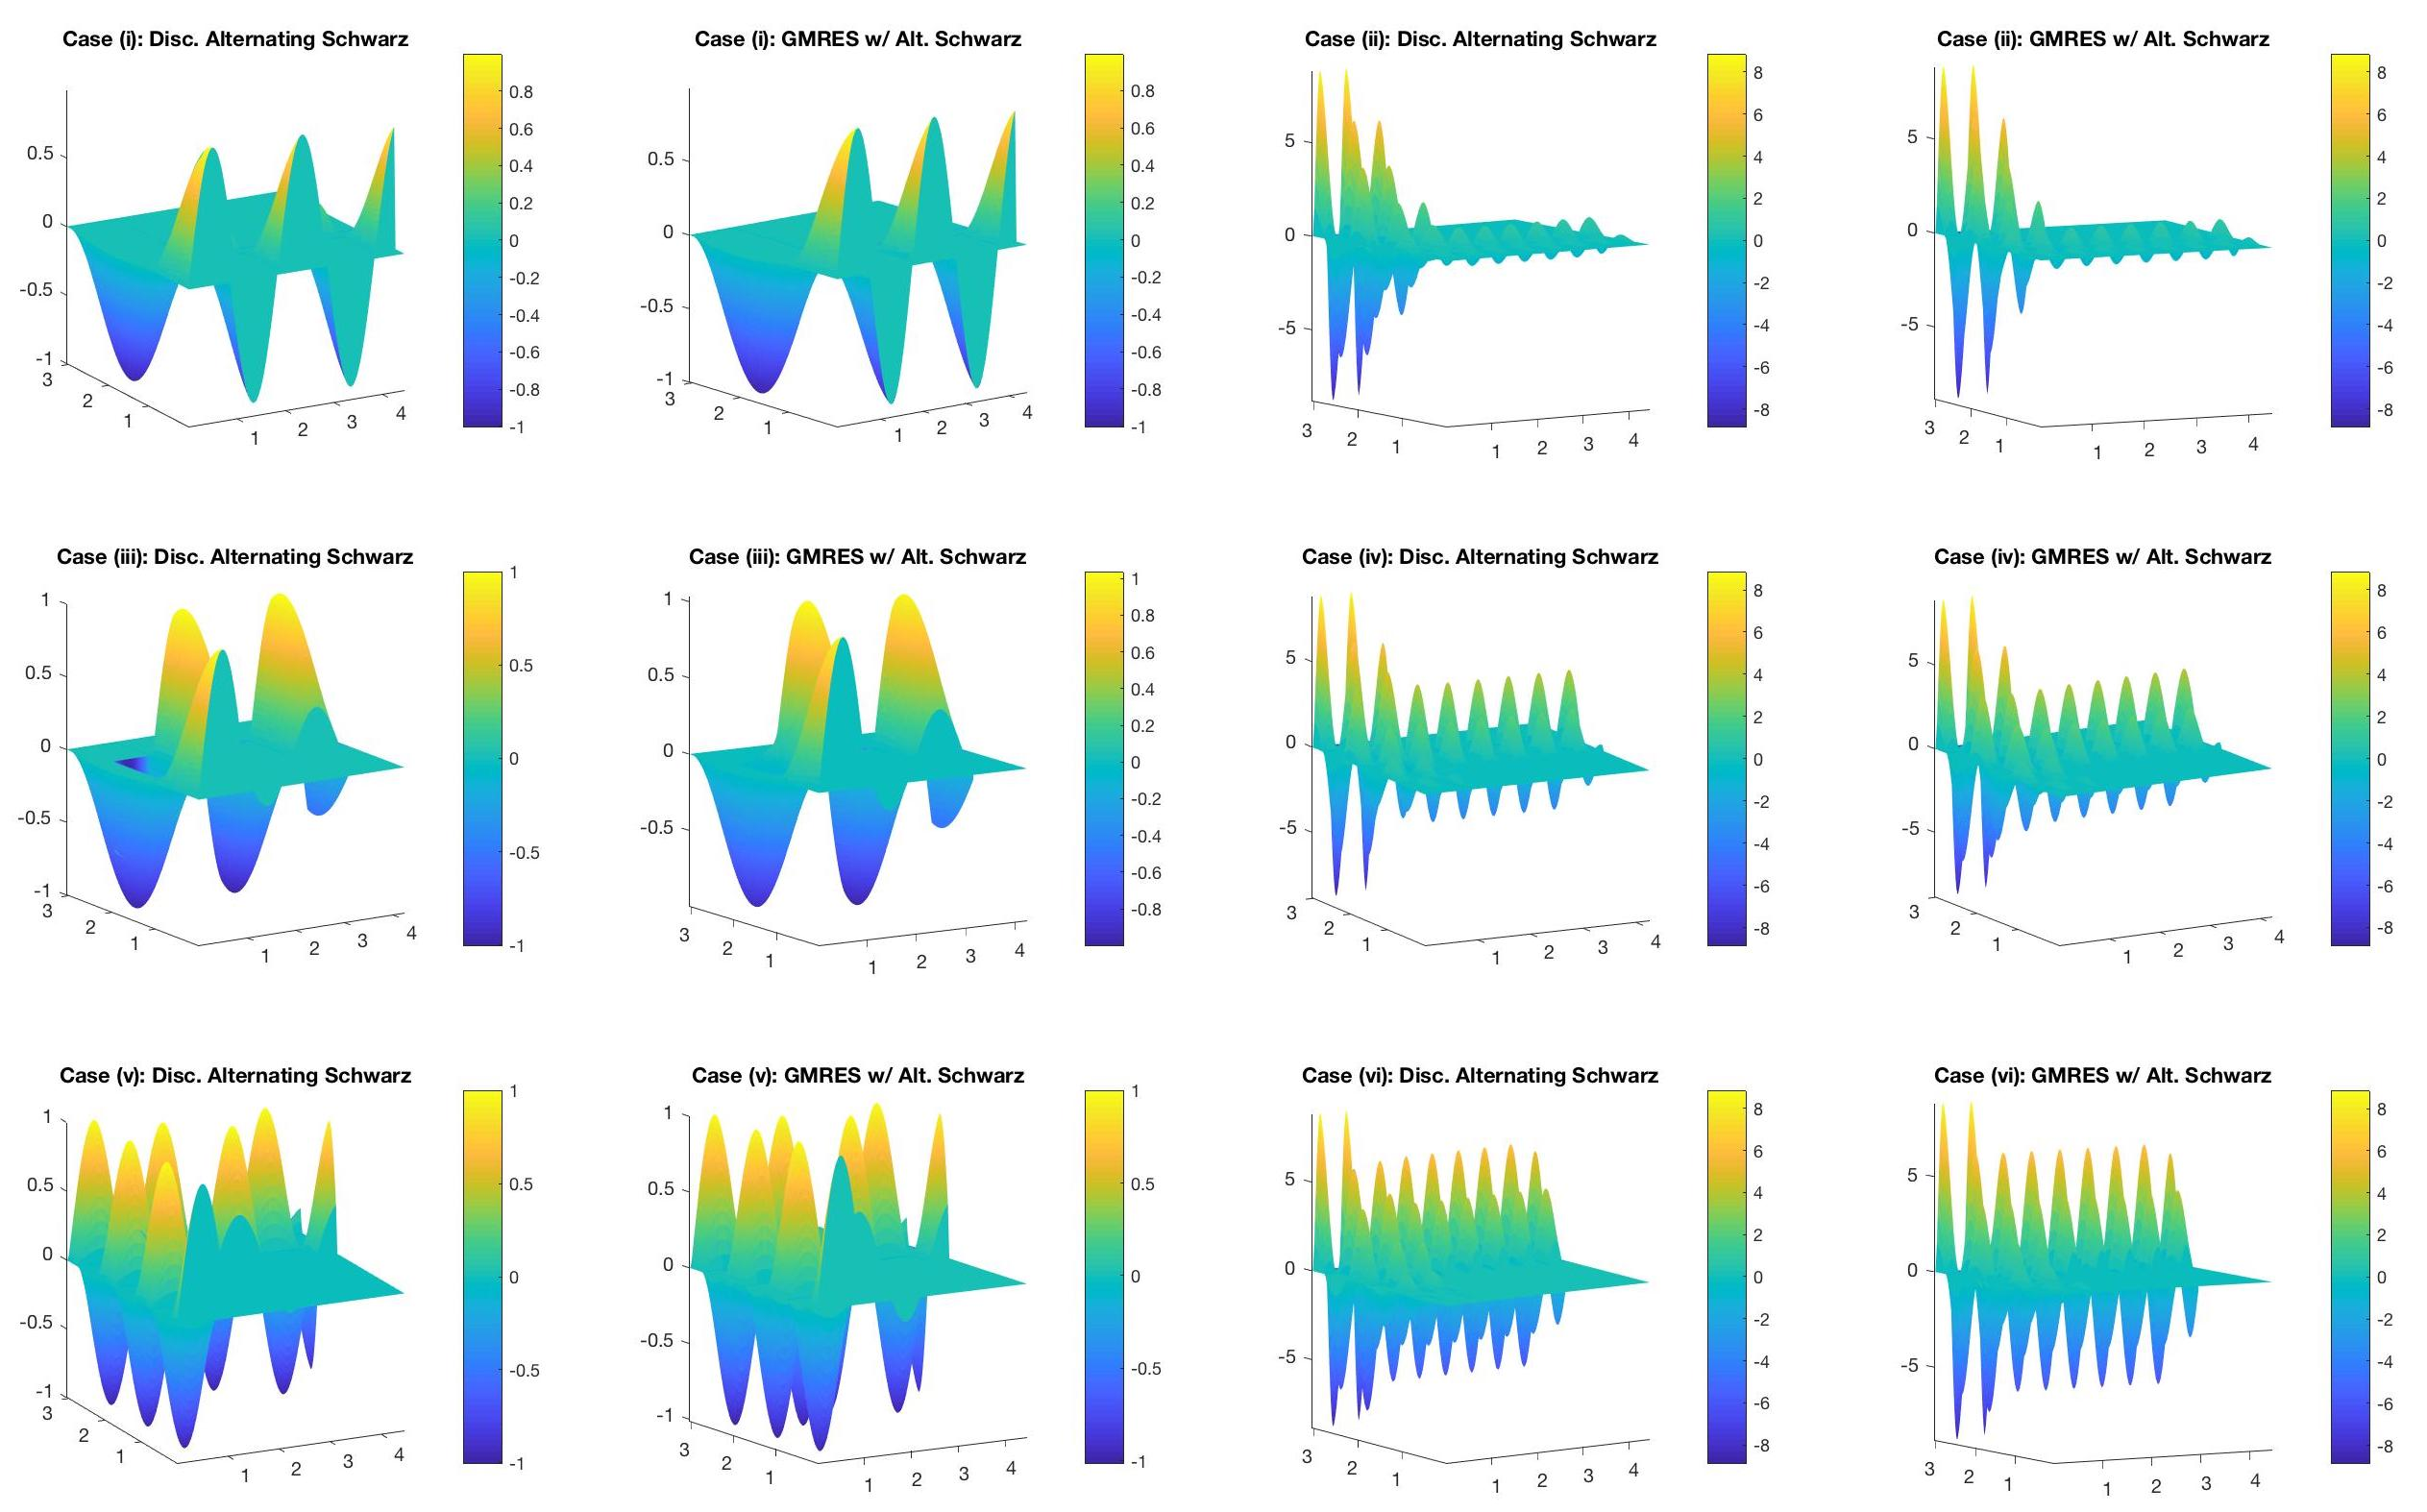
\includegraphics[scale=.23]{Part4_graphs.jpg}
\caption{Part 4 Surface Plots}
\end{figure}


\begin{table}[H]
\centering
\renewcommand{\arraystretch}{1.3}
\begin{small}
\begin{tabular}{| c || c | c | c | c | c | c | c |}
\hline
\textbf{Case} & \textbf{Method} & \textbf{m} & \textbf{tol} & \textbf{nmax} &  \textbf{Error} & \textbf{$R_1$ Solves} & \textbf{$R_2$ Solves}\\
\hline 
\hline
(i)  & DAS  & 6  & $10^{-6}$  & 100  & 1.085097526831025e-01  &  1 &  1 \\
  & GMRES  &  6 &  $10^{-6}$ & 100  &  9.402528239268292e-01 &  7 &  7 \\
\hline
(ii)  & DAS  & 6  & $10^{-6}$  & 100  & 3.390046834818040e-01  & 1  &  1 \\
  & GMRES  & 6  &  $10^{-6}$ & 100  & 3.390115972239255e-01  &  8 &  8 \\
\hline
(iii)  & DAS  & 6  & $10^{-6}$  & 100  & 1.101431531134144e-01  & 1  &  1 \\
  & GMRES  & 6  & $10^{-6}$  & 100  &  9.542182618474161e-01 &  7 & 7  \\
\hline
(iv)  &  DAS &  6 & $10^{-6}$  & 100  & 4.092714845058262e-01  & 1  &  1 \\
  & GMRES  & 6  &  $10^{-6}$ & 100  & 3.390757687521143e-01  & 8  & 8  \\
\hline
(v)  & DAS  & 6 & $10^{-6}$  & 100  &  1.961612813639500e-01 & 1  & 1  \\
  &  GMRES &  6 & $10^{-6}$  & 100  & 9.081994747619491e-01  & 7  & 7  \\
\hline
(vi)  & DAS  & 6  &  $10^{-6}$ & 100  & 6.365591205766803e-01  & 1  & 1  \\
(vi)  & GMRES  & 6  & $10^{-6}$  & 100  &  5.510901131725650e-01 &  8 & 8  \\

\hline
\end{tabular}
\end{small}
\caption{Part 4 Results}
\end{table} 

I would first like to note that I think I am calculating the error incorrectly.  I believe this is due to constructing the exact solution vector, called $\text{"u\_exact"}$ in my code, incorrectly.  Due to this problem, the error does not appear to go down as I increase $m$.  I ran out of time to figure out how to fix this, so I ran all of the cases for $m = 6$ because that is the average $m$ value that my runs in Part 3 required to converge to the actual solution with maximal residual error less than $5 \times 10^{-4}$.\\

\noindent
Also, I noticed the my surface plots for Case (v) do not exactly match the surface plots I produced in Part 3 for case (v).  I believe this error comes from one of my interpolation functions.  My guess is that the parameter values is Case (v) produce additional "special" cases of points on the artificial boundaries of $\Gamma_1$ and $\Gamma_2$ that did not arise in any of the other cases, and as such, I did not account for them in my interpolation functions.  Unfortunately, I ran out of time to investigate further.\\ 

\noindent
Now, it is a little difficult to comment on the efficiency and accuracy of my results without knowing the true error.  However, it is apparent that the Discretized Alternating Schwarz method is much more efficient since it only required one solve on $R_1$ and one solve on $R_2$ for each case.  GMRES with Alternating Schwarz Preconditioner, on the other hand, required 7 or 8 solves on $R_1$ and $R_2$ before terminating due to the tolerance being reached.





















\end{document}

% insert Matlab code
\lstset{language=matlab,frame=single}
\begin{lstlisting}[caption=]

\end{lstlisting}

% import Matlab code directly
\lstinputlisting[style=Matlab-editor,basicstyle=\ttfamily\small]{codename.m}

% OR
\lstset{language=Matlab}
\lstinputlisting{HermitianLanczos.m}

% table template
\begin{table}[H]
\centering
\renewcommand{\arraystretch}{1.3}
\begin{small}
\begin{tabular}{| c | c |}
\hline
Result &  Value\\
\hline 

\hline
\end{tabular}
\end{small}
\caption{ }
\end{table} 

% insert jpeg
\begin{figure}[H]
\center
\includegraphics[scale=.39]{ .jpg}
\caption{ }
\end{figure}

% negative hspace - move figures/tables/etc over to the left
\hspace{-.5in}


% change text color
{\color{red} **colored text goes here}

% change the text size in math environment
\[\Scale[0.5]{y = \sin^2 x}\] 

% to put a colored box around something. can change color
\begin{mybox}{red}{Title}
Stuff in box
\end{mybox}

% put default colored box around something
\begin{tcolorbox}
Stuff in box
\end{tcolorbox}